% Options for packages loaded elsewhere
\PassOptionsToPackage{unicode}{hyperref}
\PassOptionsToPackage{hyphens}{url}
\PassOptionsToPackage{dvipsnames,svgnames,x11names}{xcolor}
%
\documentclass[
]{agujournal2019}

\usepackage{amsmath,amssymb}
\usepackage{iftex}
\ifPDFTeX
  \usepackage[T1]{fontenc}
  \usepackage[utf8]{inputenc}
  \usepackage{textcomp} % provide euro and other symbols
\else % if luatex or xetex
  \usepackage{unicode-math}
  \defaultfontfeatures{Scale=MatchLowercase}
  \defaultfontfeatures[\rmfamily]{Ligatures=TeX,Scale=1}
\fi
\usepackage{lmodern}
\ifPDFTeX\else  
    % xetex/luatex font selection
\fi
% Use upquote if available, for straight quotes in verbatim environments
\IfFileExists{upquote.sty}{\usepackage{upquote}}{}
\IfFileExists{microtype.sty}{% use microtype if available
  \usepackage[]{microtype}
  \UseMicrotypeSet[protrusion]{basicmath} % disable protrusion for tt fonts
}{}
\makeatletter
\@ifundefined{KOMAClassName}{% if non-KOMA class
  \IfFileExists{parskip.sty}{%
    \usepackage{parskip}
  }{% else
    \setlength{\parindent}{0pt}
    \setlength{\parskip}{6pt plus 2pt minus 1pt}}
}{% if KOMA class
  \KOMAoptions{parskip=half}}
\makeatother
\usepackage{xcolor}
\setlength{\emergencystretch}{3em} % prevent overfull lines
\setcounter{secnumdepth}{-\maxdimen} % remove section numbering
% Make \paragraph and \subparagraph free-standing
\makeatletter
\ifx\paragraph\undefined\else
  \let\oldparagraph\paragraph
  \renewcommand{\paragraph}{
    \@ifstar
      \xxxParagraphStar
      \xxxParagraphNoStar
  }
  \newcommand{\xxxParagraphStar}[1]{\oldparagraph*{#1}\mbox{}}
  \newcommand{\xxxParagraphNoStar}[1]{\oldparagraph{#1}\mbox{}}
\fi
\ifx\subparagraph\undefined\else
  \let\oldsubparagraph\subparagraph
  \renewcommand{\subparagraph}{
    \@ifstar
      \xxxSubParagraphStar
      \xxxSubParagraphNoStar
  }
  \newcommand{\xxxSubParagraphStar}[1]{\oldsubparagraph*{#1}\mbox{}}
  \newcommand{\xxxSubParagraphNoStar}[1]{\oldsubparagraph{#1}\mbox{}}
\fi
\makeatother


\providecommand{\tightlist}{%
  \setlength{\itemsep}{0pt}\setlength{\parskip}{0pt}}\usepackage{longtable,booktabs,array}
\usepackage{calc} % for calculating minipage widths
% Correct order of tables after \paragraph or \subparagraph
\usepackage{etoolbox}
\makeatletter
\patchcmd\longtable{\par}{\if@noskipsec\mbox{}\fi\par}{}{}
\makeatother
% Allow footnotes in longtable head/foot
\IfFileExists{footnotehyper.sty}{\usepackage{footnotehyper}}{\usepackage{footnote}}
\makesavenoteenv{longtable}
\usepackage{graphicx}
\makeatletter
\def\maxwidth{\ifdim\Gin@nat@width>\linewidth\linewidth\else\Gin@nat@width\fi}
\def\maxheight{\ifdim\Gin@nat@height>\textheight\textheight\else\Gin@nat@height\fi}
\makeatother
% Scale images if necessary, so that they will not overflow the page
% margins by default, and it is still possible to overwrite the defaults
% using explicit options in \includegraphics[width, height, ...]{}
\setkeys{Gin}{width=\maxwidth,height=\maxheight,keepaspectratio}
% Set default figure placement to htbp
\makeatletter
\def\fps@figure{htbp}
\makeatother
% definitions for citeproc citations
\NewDocumentCommand\citeproctext{}{}
\NewDocumentCommand\citeproc{mm}{%
  \begingroup\def\citeproctext{#2}\cite{#1}\endgroup}
\makeatletter
 % allow citations to break across lines
 \let\@cite@ofmt\@firstofone
 % avoid brackets around text for \cite:
 \def\@biblabel#1{}
 \def\@cite#1#2{{#1\if@tempswa , #2\fi}}
\makeatother
\newlength{\cslhangindent}
\setlength{\cslhangindent}{1.5em}
\newlength{\csllabelwidth}
\setlength{\csllabelwidth}{3em}
\newenvironment{CSLReferences}[2] % #1 hanging-indent, #2 entry-spacing
 {\begin{list}{}{%
  \setlength{\itemindent}{0pt}
  \setlength{\leftmargin}{0pt}
  \setlength{\parsep}{0pt}
  % turn on hanging indent if param 1 is 1
  \ifodd #1
   \setlength{\leftmargin}{\cslhangindent}
   \setlength{\itemindent}{-1\cslhangindent}
  \fi
  % set entry spacing
  \setlength{\itemsep}{#2\baselineskip}}}
 {\end{list}}
\usepackage{calc}
\newcommand{\CSLBlock}[1]{\hfill\break\parbox[t]{\linewidth}{\strut\ignorespaces#1\strut}}
\newcommand{\CSLLeftMargin}[1]{\parbox[t]{\csllabelwidth}{\strut#1\strut}}
\newcommand{\CSLRightInline}[1]{\parbox[t]{\linewidth - \csllabelwidth}{\strut#1\strut}}
\newcommand{\CSLIndent}[1]{\hspace{\cslhangindent}#1}

\usepackage{url} %this package should fix any errors with URLs in refs.
\usepackage{lineno}
\usepackage[inline]{trackchanges} %for better track changes. finalnew option will compile document with changes incorporated.
\usepackage{soul}
\linenumbers
\makeatletter
\@ifpackageloaded{caption}{}{\usepackage{caption}}
\AtBeginDocument{%
\ifdefined\contentsname
  \renewcommand*\contentsname{Table of contents}
\else
  \newcommand\contentsname{Table of contents}
\fi
\ifdefined\listfigurename
  \renewcommand*\listfigurename{List of Figures}
\else
  \newcommand\listfigurename{List of Figures}
\fi
\ifdefined\listtablename
  \renewcommand*\listtablename{List of Tables}
\else
  \newcommand\listtablename{List of Tables}
\fi
\ifdefined\figurename
  \renewcommand*\figurename{Figure}
\else
  \newcommand\figurename{Figure}
\fi
\ifdefined\tablename
  \renewcommand*\tablename{Table}
\else
  \newcommand\tablename{Table}
\fi
}
\@ifpackageloaded{float}{}{\usepackage{float}}
\floatstyle{ruled}
\@ifundefined{c@chapter}{\newfloat{codelisting}{h}{lop}}{\newfloat{codelisting}{h}{lop}[chapter]}
\floatname{codelisting}{Listing}
\newcommand*\listoflistings{\listof{codelisting}{List of Listings}}
\makeatother
\makeatletter
\makeatother
\makeatletter
\@ifpackageloaded{caption}{}{\usepackage{caption}}
\@ifpackageloaded{subcaption}{}{\usepackage{subcaption}}
\makeatother

\ifLuaTeX
  \usepackage{selnolig}  % disable illegal ligatures
\fi
\usepackage{bookmark}

\IfFileExists{xurl.sty}{\usepackage{xurl}}{} % add URL line breaks if available
\urlstyle{same} % disable monospaced font for URLs
\hypersetup{
  pdftitle={Cumulative and individual impacts of the human footprint on biodiversity indicators using dissimilarity to high integrity reference states.},
  pdfauthor={Evan Muise; Nicholas Coops; Txomin Hermosilla; Chris Mulverhill; Cole Burton; Stephen Ban},
  pdfkeywords={Protected areas, Coarsened exact matching, Reference
states, Remote sensing, Ecosystem structure, Ecosystem
function, Anthropogenic pressure, Human footprint},
  colorlinks=true,
  linkcolor={blue},
  filecolor={Maroon},
  citecolor={Blue},
  urlcolor={Blue},
  pdfcreator={LaTeX via pandoc}}



\draftfalse

\begin{document}
\title{Cumulative and individual impacts of the human footprint on
biodiversity indicators using dissimilarity to high integrity reference
states.}

\authors{Evan Muise\affil{1}, Nicholas Coops\affil{1}, Txomin
Hermosilla\affil{2}, Chris Mulverhill\affil{1}, Cole
Burton\affil{1}, Stephen Ban\affil{3}}
\affiliation{1}{Department of Forest Resource Management, University of
British Columbia, Vancouver, British Columbia,
Canada, }\affiliation{2}{Canadian Forest Service (Pacific Forestry
Centre), Natural Resources Canada, Victoria, British Columbia,
Canada, }\affiliation{3}{BC Parks, Government of British Columbia,
Victoria, British Columbia, Canada, }
\correspondingauthor{Evan Muise}{evanmuis@student.ubc.ca}







\section{Abstract}\label{abstract}

Forests with high ecological integrity are incredibly important for
biodiversity conservation, and provide integral ecosystem services.
These forests have natural or near-natural ecosystem structure,
function, and composition. Anthropogenic pressures such as habitat loss,
overexploitation of natural resources, and land use changes are leading
to the degradation or loss of high-integrity forests. As a result,
assessing forest integrity over large areas is increasingly important
for a range of conservation initiatives. Recently, we have seen an
increase in the application of remote sensing data to assess a range of
forest structural and functional attributes, which can provide insights
into forest integrity through space and time. In this study, we use
satellite-derived forest structural attributes and forest functioning
metrics alongside a high-quality reference state to calculate ecological
dissimilarity as a proxy for ecological integrity. We further refine our
reference states by using coarsened exact matching to ensure our
comparisons are drawn from suitable protected analogs. We applied these
methods onto Vancouver Island, Canada, where we assessed how far, in
structural and functional space, forest stands were from reference,
high-integrity forests found in the island's oldest and largest
protected area. We further assess how individual and cumulative
anthropogenic pressure are influencing the ecological integrity of
forests on the island. We found that forest structural dissimilarity
increased under high levels of anthropogenic pressures (ANOVA; p
\textless{} 0.01), while functional dissimilarity was not impacted by
any anthropogenic pressures (ANOVA; p \textgreater{} 0.05). For
individual pressures, we found that built environments, harvesting, and
population density influenced structural dissimilarity (ANOVA; p
\textless{} 0.05), while roads did not influence structural
dissimilarity (ANOVA; p \textgreater{} 0.05). These types of methods can
be used to identify high-integrity forest ecosystems which should be
prioritized for protection, or to identify areas with low levels of
pressures which could benefit from restoration efforts, helping move
towards the Kunming-Montreal Global Biodiversity Framework's goal of
30\% of all ecosystems protected, with a focus on high-integrity
ecosystems

\section{Introduction}\label{introduction}

In the terrestrial environment, forests have been shown to possess
larges amounts of biodiversity (Cardinale et al., 2012; Myers, 1988;
Pimm and Raven, 2000) and provide key ecosystem services (Thompson et
al., 2009). However, the ongoing impact of anthropogenic pressures such
as climate change, overexploitation of natural resources, and invasive
species are leading to forest degradation, reducing the ability of
forested ecosystems to provide these services (Thomas et al., 2004;
Urban, 2015). Therefore it is integral to maintain and conserve forests
that are in good ecological condition, as defined by natural or
near-natural levels of forest structure, function, and composition,
often referred to as having high ecological integrity (Marín et al.,
2021). The importance of high-integrity ecosystems has led to a general
call to move beyond simple quantification of ecosystem or forest extent
in conservation strategies to other metrics which additionally consider
the integrity of the conserved ecosystem (Ferrier et al., 2024; Hansen
et al., 2020; Muise et al., 2022; Pillay et al., 2024a). In December
2022, the Kunming-Montreal Global Biodiversity Framework (GBF) was
adopted with the goal of restoring and safeguarding global biodiversity
(Convention on Biological Diversity, 2023). Targets within this
framework include restoring 30\% of all degraded ecosystems, protecting
30\% of the Earth's terrestrial, inland water, and marine areas by 2030,
and achieving no loss of high biodiversity importance areas, especially
high ecological integrity ecosystems (Convention on Biological
Diversity, 2023). However, there are currently no spatially explicitly
assessments of ecological integrity available at the regional or larger
scale, making progress towards these goals difficult to quantify.

Assessing ecological integrity requires a comprehensive evaluation of
ecosystem structure, function, and composition, which can be effectively
achieved using remote sensing-derived indicators (Pereira et al., 2013;
Radeloff et al., 2024; Skidmore et al., 2021). Advances in remote
sensing technologies such as light detection and ranging (lidar) allow
for the accurate measurement of forest structural attributes, including
canopy height, canopy cover, vertical complexity, and biomass (Bergen et
al., 2009; Valbuena et al., 2020). These indicators of forest structure
can provide critical insights into habitat quality and the capacity of
ecosystems to support biodiversity (Gao et al., 2014; Guo et al., 2017;
Macarthur and Macarthur, 1961), and are rapidly becoming available at
the national scale through new modelling methods (Matasci et al., 2018a;
Matasci et al., 2018b; Potapov et al., 2021). Additionally, remote
sensing facilitates the monitoring of functional processes, such as
photosynthetic activity and forest phenology, through the use of
spectral indices such as the normalized difference vegetation index
(NDVI) (Pettorelli et al., 2018, 2005), amongst others. By integrating
these indices over the course of the year, it is possible to assess the
energy availability, seasonality, and stress on an ecosystem (Radeloff
et al., 2019; Razenkova, 2023), which have also been shown to be linked
to biodiversity in a variety of taxa (Andrew et al., 2024, 2012; Coops
et al., 2019, 2009b; Razenkova et al., 2022). Further, structural and
functional indicators have been shown to have low information overlap
(Muise et al., 2024), thereby making it suitable use satellite-derived
structural and functional indicators to assess ecological integrity
across regions, countries, or even continents by comparing them to a
suitable reference state (Grantham et al., 2020; Hansen et al., 2020).

Another key aspect of assessing ecological integrity is the reference
state, typically defined as an example of an ecosystem that has not been
subject major anthropogenic disturbance (Hansen et al., 2020; Nicholson
et al., 2021). These reference states represent the baseline conditions
of ecosystems and serve as a benchmark for assessing ecological health
and guiding protection and restoration efforts (Nielsen et al., 2007). A
number of methods have been proposed for identifying reference states,
including protected areas (Arcese and Sinclair, 1997), historical
(McNellie et al., 2020), and empirical reference states (Ferraro, 2009;
Nielsen et al., 2007). Protected area reference states are commonly used
because conservation efforts aim to mitigate anthropogenic pressures
within protected areas (Geldmann et al., 2019), and the bias for
protected areas to be placed in areas with low amounts of anthropogenic
pressures (Joppa and Pfaff, 2009) and less productive land covers (Muise
et al., 2022). Due to the bias in protected area placement, it is
necessary to account for differences in environmental conditions and
land covers when using them as a reference state, which is typically
accomplished using counterfactual methods (Ferraro, 2009), such as
coarsened exact matching (Iacus et al., 2012). Using these methods it
becomes possible to identify a suitable reference state for the entirety
of a region, by comparing to protected areas without anthropogenic
pressure under similar environmental conditions and land covers.

Building on this foundation, the objective of this study is to develop
and implement a spatially explicit framework for assessing ecological
integrity at regional to continental scales using remote sensing data.
Specifically, we aim to (1) integrate satellite-derived indicators of
forest structure and function with robust counterfactual methods to
establish reference states, (2) quantify deviations from these reference
states as a measure of ecological degradation, and (3) demonstrate the
utility of this method across a regional study area. This work addresses
a critical gap in the operationalization of global biodiversity targets,
such as those outlined in the GBF, by providing a scalable, reproducible
approach to monitor and guide conservation and restoration efforts. By
enabling the identification of areas with high ecological integrity and
those most in need of restoration, this study has the potential to
directly inform policy and support more effective biodiversity
conservation strategies.

\section{Methods}\label{methods}

To accomplish our objectives, we propose a novel, data-driven approach
to identify high-integrity forests based on various satellite derived
metrics of ecosystem condition. First, we account for differences in
environmental conditions by implementing a coarsened exact matching
approach (Iacus et al., 2012). This ensures that ecosystems must be
similar to their protected counterparts (i.e.~a forest in a valley
bottom and a mountain top would not be compared to one another), which
accounts for biases in protected area placement (Joppa and Pfaff, 2009;
Muise et al., 2022). We use the sigma dissimilarity metric (Mahony et
al., 2017) to calculate the similarity to high-integrity, undisturbed,
forests in both structural and functional space as a metric of
ecological integrity. Finally, we validate our results by assessing the
impact anthropogenic pressures (Hirsh-Pearson et al., 2022) on our
similarity metric, with the assumption that increased anthropogenic
pressures should increase ecological dissimilarity. We focus our study
area on Vancouver Island, British Columbia, Canada, as a case study and
demonstration of the method.

\subsection{Study Area}\label{sec-study}

We focus on the forested areas of Vancouver Island, British Columbia,
Canada. Vancouver Island has approximately 31,285 km\textsuperscript{2}
of land area, of which 79.5\% is forested. The dominant forest species
on Vancouver Island are Douglas-fir (\emph{Pseudotsuga menziesii}),
western red cedar (\emph{Thuja plicata}), western hemlock (\emph{Tsuga
heterophylla}), yellow cedar (\emph{Chamaecyparis nootkatensis}), and
Sitka spruce (\emph{Picea sitchensis}) (Burns, 1990). Vancouver Island
generally has a temperate maritime climate, with mild, wet winters, and
cool, dry summers. There are four ecosystems on Vancouver Island as
defined by British Columbia's biogeoclimatic ecosystem classification
(BEC) framework (Pojar et al., 1987), Coastal Western Hemlock (CWH),
Mountain Hemlock (MH), Coastal Douglas Fir (CDF), and Coastal
Mountain-heather Alpine (CMA), which are broadly delineated based on
soil, climate, and elevation. Forestry is an important industry on
Vancouver Island, with the majority of the land base being managed for
timber production under various tenures, including private ownership
(Ministry of Water, Land and Resource Stewardship (WLRS), 2023). These
harvesting practices have led to a need to protect remaining
high-integrity forests, and restore degraded forests. Fires on Vancouver
Island have historically been infrequently and of low severity (Daniels
and Gray, 2006).

\subsubsection{Reference State}\label{reference-state}

Strathcona Park provided an exceptional reference state for the
undisturbed forest ecosystems on Vancouver Island due to its
long-standing protection and large size. Established in 1911 as the
oldest and largest provincial park in British Columbia, it encompasses
2,480 km², with approximately 80\% designated as wilderness and Nature
Conservancy Areas under the Park Act ({``Park {Act},''} 1996). These
designations have ensured the preservation of natural ecological
processes, leaving the park relatively free from anthropogenic
disturbances over more than a century. Strathcona Park includes three of
the island's BEC zones: CWH, MH, and CMA. However, the CDF zone, limited
to the southern part of Vancouver Island and subject to extensive
anthropogenic alteration, is not represented within the park. As such,
we do not include CDF in our analysis. By focusing on undisturbed
forests within Strathcona Park as a reference state, our analysis
prioritizes areas of minimal human impact and ecological continuity,
providing a robust benchmark for assessing forest ecosystems in their
natural state.

\phantomsection\label{cell-fig-study}
\begin{figure}[H]

\centering{

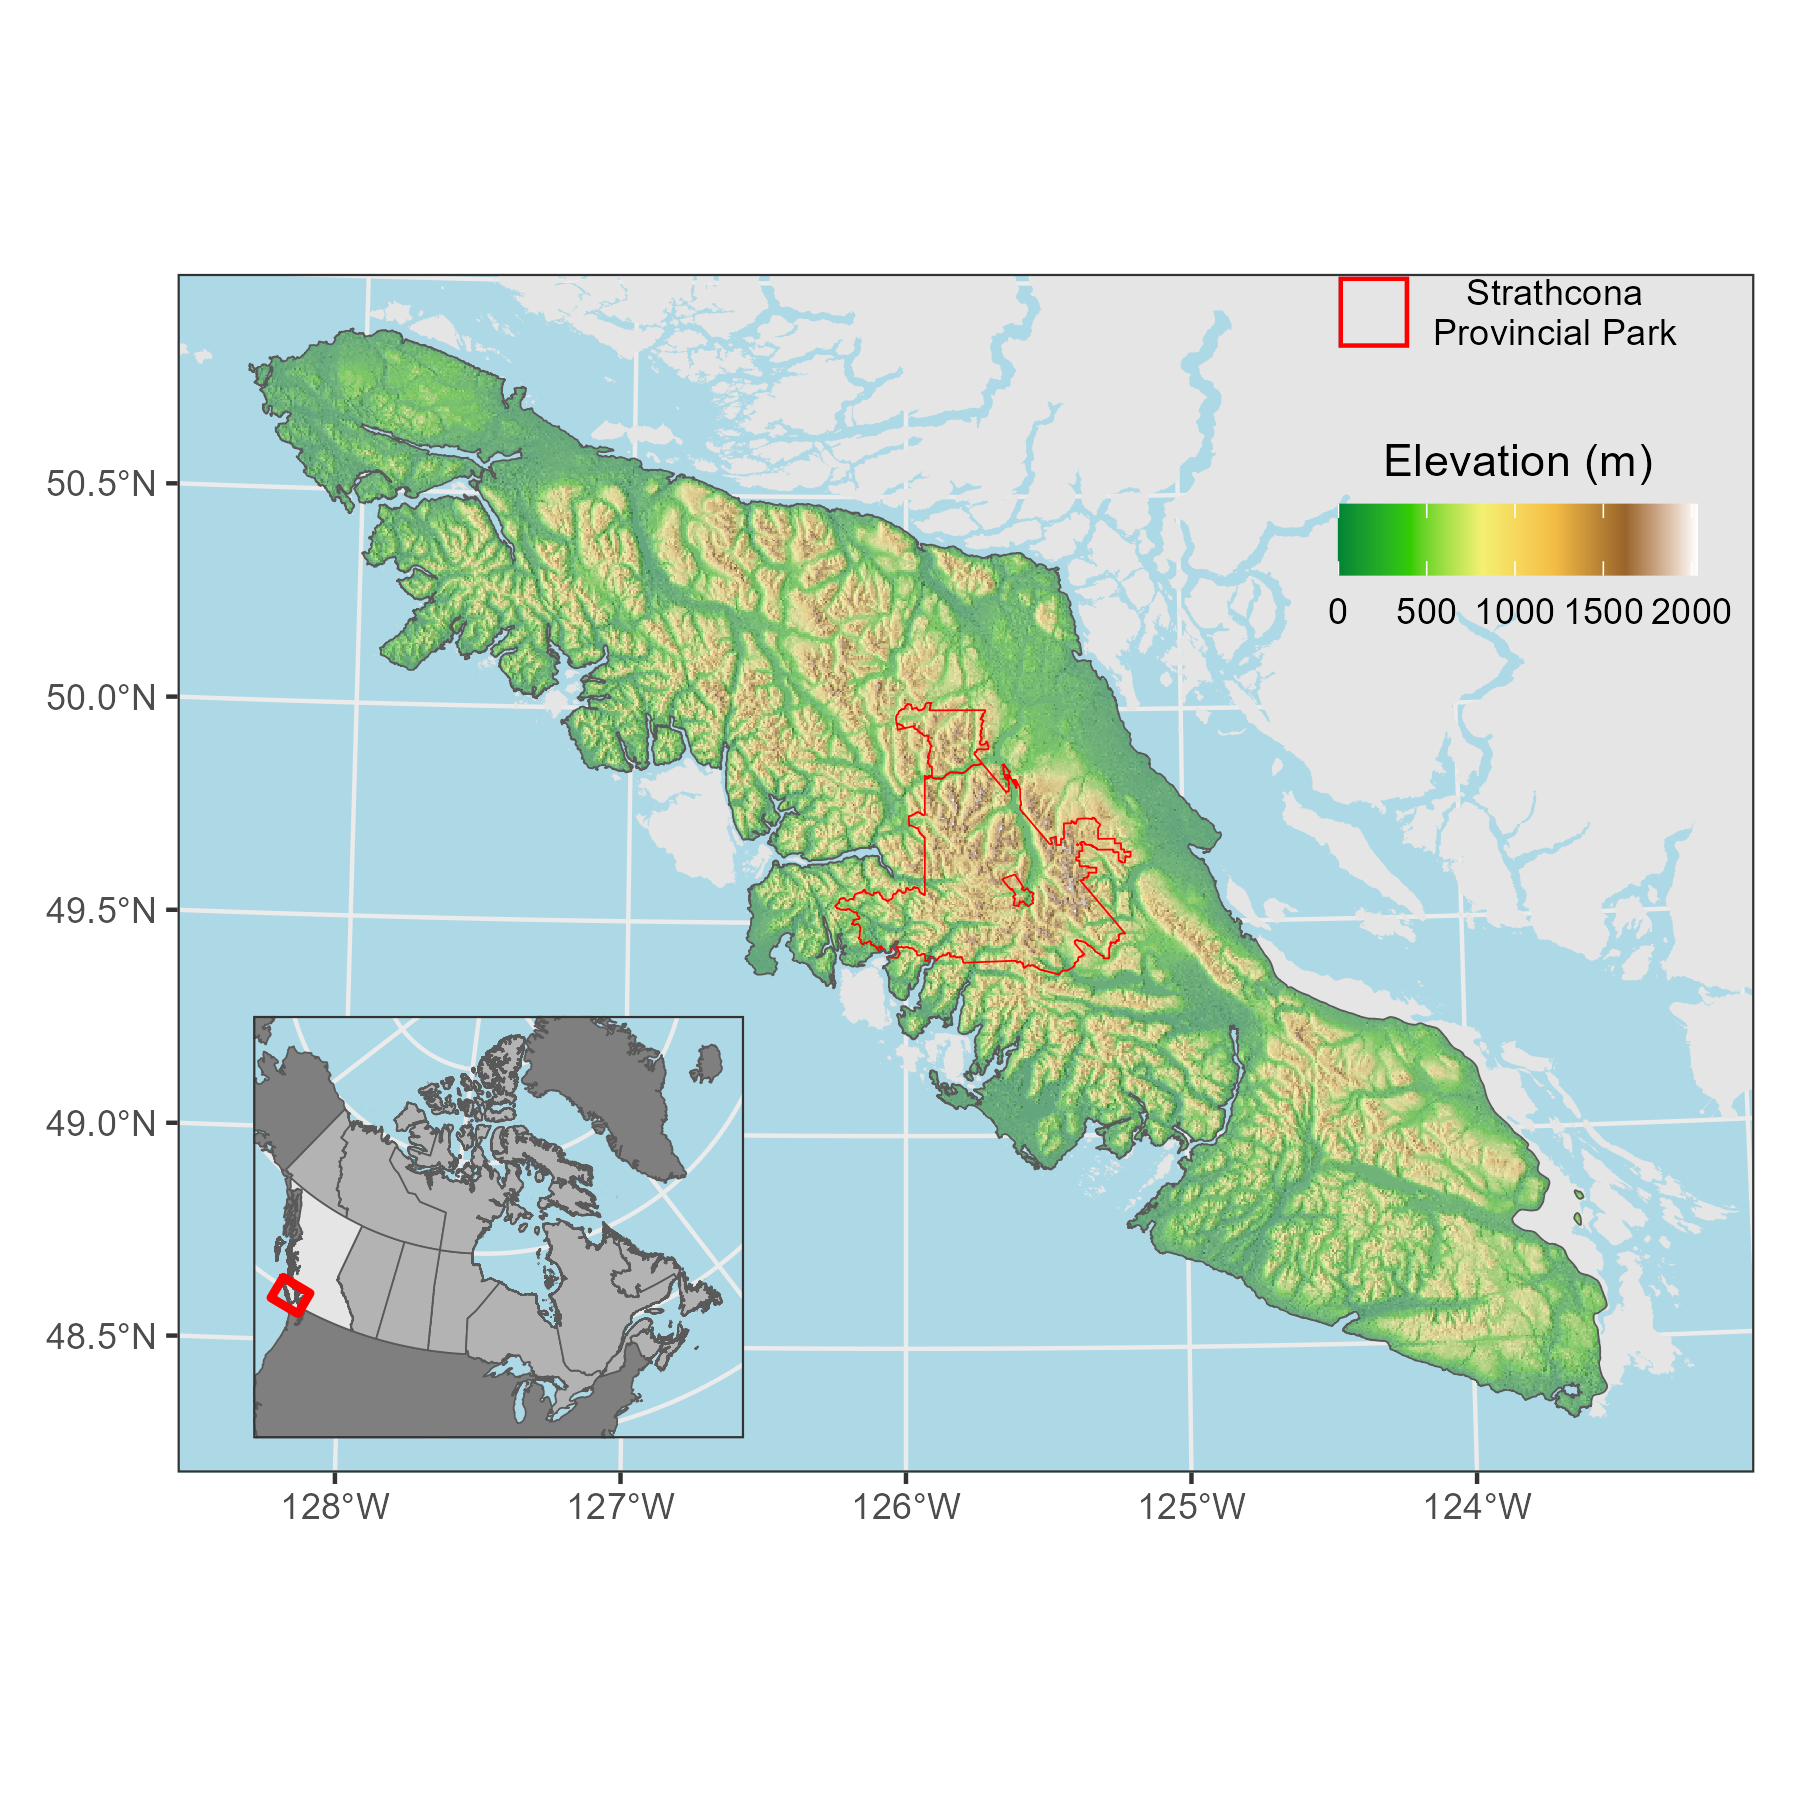
\includegraphics[width=6in,height=\textheight]{figures/study_area.png}

}

\caption{\label{fig-study}Study area on Vancouver Island, British
Columbia, Canada, including the location of Strathcona Provincial Park.}

\end{figure}%

\subsection{Data}\label{data}

\subsubsection{Forest Structure}\label{forest-structure}

We utilize four forest structural attributes; canopy height, canopy
cover, structural complexity, and aboveground biomass. Canopy height,
canopy cover, structural complexity are standardized lidar-derived
metrics suitable for biodiversity monitoring at the ecosystem scale
(Valbuena et al., 2020). These are commonly used to assess patterns of
structure in the vertical and horizontal directions within a single
stand, rather than across a landscape, with these stand level metrics
being linked to habitat, and thus, biodiversity (Bergen et al., 2009;
Gao et al., 2014; Macarthur and Macarthur, 1961). The fourth attribute,
aboveground biomass, represents the key ecosystem service of carbon
sequestration (Duncanson et al., 2023; Naidoo and Ricketts, 2006), and
is likely moderated by the three lidar-derived variables (Ali, 2019).

These four forest structural attributes were generated in a wall-to-wall
fashion at a 30 m spatial resolution by Matasci et al. (2018a) for the
year 2015 using a random forest-kNN approach, that imputes lidar-derived
forest structural attributes across Canada's forested ecosystems using
Landsat-derived best-available-pixel (BAP) composites (Hermosilla et
al., 2016; White et al., 2014) and topographic information (Matasci et
al., 2018a; Matasci et al., 2018b). The BAP composites were generated by
selecting surface reflectance observations from the Landsat archive over
the course of Canada's growing season (August 1\textsuperscript{st} ± 30
days), avoiding atmospheric effects including haze, clouds, and cloud
shadows These composites were further refined by using a spectral trend
analysis remove noise and infill data gaps (Hermosilla et al., 2015).
Accuracy metrics for the forest structural attributes ranged from an
RMSE of 29.7\% (structural complexity) to 65.8\% (aboveground biomass)
and R\textsuperscript{2} values of 0.70 (aboveground biomass) to 0.13
(structural complexity).

\subsubsection{Forest Function}\label{forest-function}

To represent forest ecosystem function, we use the Dynamic Habitat
Indices (DHIs) dataset, a suite of intra-annual summaries of energy (as
represented by a vegetation index or estimate of gross/net primary
productivity) availability (Radeloff et al., 2019). Single time points
of energy availability have commonly been used as indicators of
ecosystem functioning (Pettorelli et al., 2018, 2005), and the DHIs
advance upon these snapshots by generating yearly summaries of energy
availability, thus more strongly linking these metrics to ecosystem
functioning. The DHIs are composed of the total available energy over
the course of a year (Cumulative DHI), the minimum amount of energy
available over the course of a year (Minimum DHI), and the variation in
energy available over the course of a year (Variation DHI). The DHIs
have been shown to be indicative of ecosystem functioning, as they
represent energy availability and seasonality (Berry et al., 2007), and
biodiversity over a range of scales (Radeloff et al., 2019; Razenkova et
al., 2022), extents (Coops et al., 2019, 2009a) and taxa (Michaud et
al., 2014; Suttidate et al., 2021).

We calculated the DHIs at a 30 m spatial resolution using Landsat data,
following the methodology of Razenkova (2023). The DHIs were computed on
Google Earth Engine (Gorelick et al., 2017) by creating a synthetic year
of monthly NDVI composites using all available Landsat imagery from
2011-2020 (centred on 2015). We used the Landsat QA band (Zhu and
Woodcock, 2012) to filter pixels with clouds and cloud shadows. Monthly
NDVI values were calculated by taking the median of each month's NDVI
observations, ignoring the year the image was acquired. This resulted in
DHIs at 30 m spatial resolution (Razenkova, 2023). The DHIs are
calculated as the sum (Cumulative DHI), minimum (Minimum DHI), and
coefficient of variation (Variation DHI) of these monthly observations.
In this study, we focus on the Cumulative and Variation DHIs, as the
minimum DHI is consistently 0 due to the presence of snow during winter
in our study area.

\subsubsection{Anthropogenic Pressures}\label{anthropogenic-pressures}

We used the Canadian Human Footprint as developed by Hirsh-Pearson et
al. (2022) to indicate anthropogenic pressures on the environment. The
Canadian Human Footprint is an additive pressure map generated by
summing the 12 different anthropogenic pressures (built environments,
crop land, pasture land, population density, nighttime lights, railways,
roads, navigable waterways, dams and associated reservoirs, mining
activity, oil and gas, and forestry), which ranges from zero to 55 for
any cell across Canada. This cumulative dataset is also distributed with
Canada-wide individual pressure values (Hirsh-Pearson et al., n.d.). We
use the anthropogenic pressure layers to define our reference state by
excluding pixels with any amount of anthropogenic pressure in Strathcona
Park, and also assess the impact of anthropogenic pressures on
ecological integrity. Here, we focus on the overall cumulative pressure
map and four individual pressures: population density, built
environments, roads, and forestry. We selected these four as other
pressures (oil and gas; railroads) are not present on Vancouver Island,
while pasture land and crop land do not coincide with currently forested
areas. We reclassify the Canadian Human Footprint (Hirsh-Pearson et al.,
n.d.; Hirsh-Pearson et al., 2022) into categorical data following
Hirsh-Pearson et al. (2022) and Arias-Patino et al. (2024): a value of
zero is considered intact, zero to four has low anthropogenic pressure,
four to eight has medium anthropogenic pressure, and above eight has
high anthropogenic pressure.

\subsubsection{Covariates}\label{covariates}

In order to ensure that we were identifying suitable reference states,
we matched undisturbed forest areas within Strathcona Park with forested
areas outside the park based on topographic and climatic features. We
use a 30 m digital elevation model and derived slope dataset from the
Advanced Spaceborne Thermal Emission and Reflection Radiometer (ASTER)
Version 3 GDEM product (Abrams et al., 2020). We also used four climate
variables; mean annual precipitation (MAP), mean annual temperature
(MAT), mean warmest month temperature (MWMT), and mean coldest month
temperature (MCMT) calculated from 1990-2020 climate normals using the
ClimateNA software package at a 1 km spatial resolution, and downsampled
to 30 m using cubic spline resampling in the \textbf{terra} (version
1.7-71) R package (Hijmans, 2024) in R (R Core Team, 2024 version
4.4.1). A visualization of one of each input dataset can be found in
Figure~\ref{fig-data}.

\phantomsection\label{cell-fig-data}
\begin{figure}[H]

\centering{

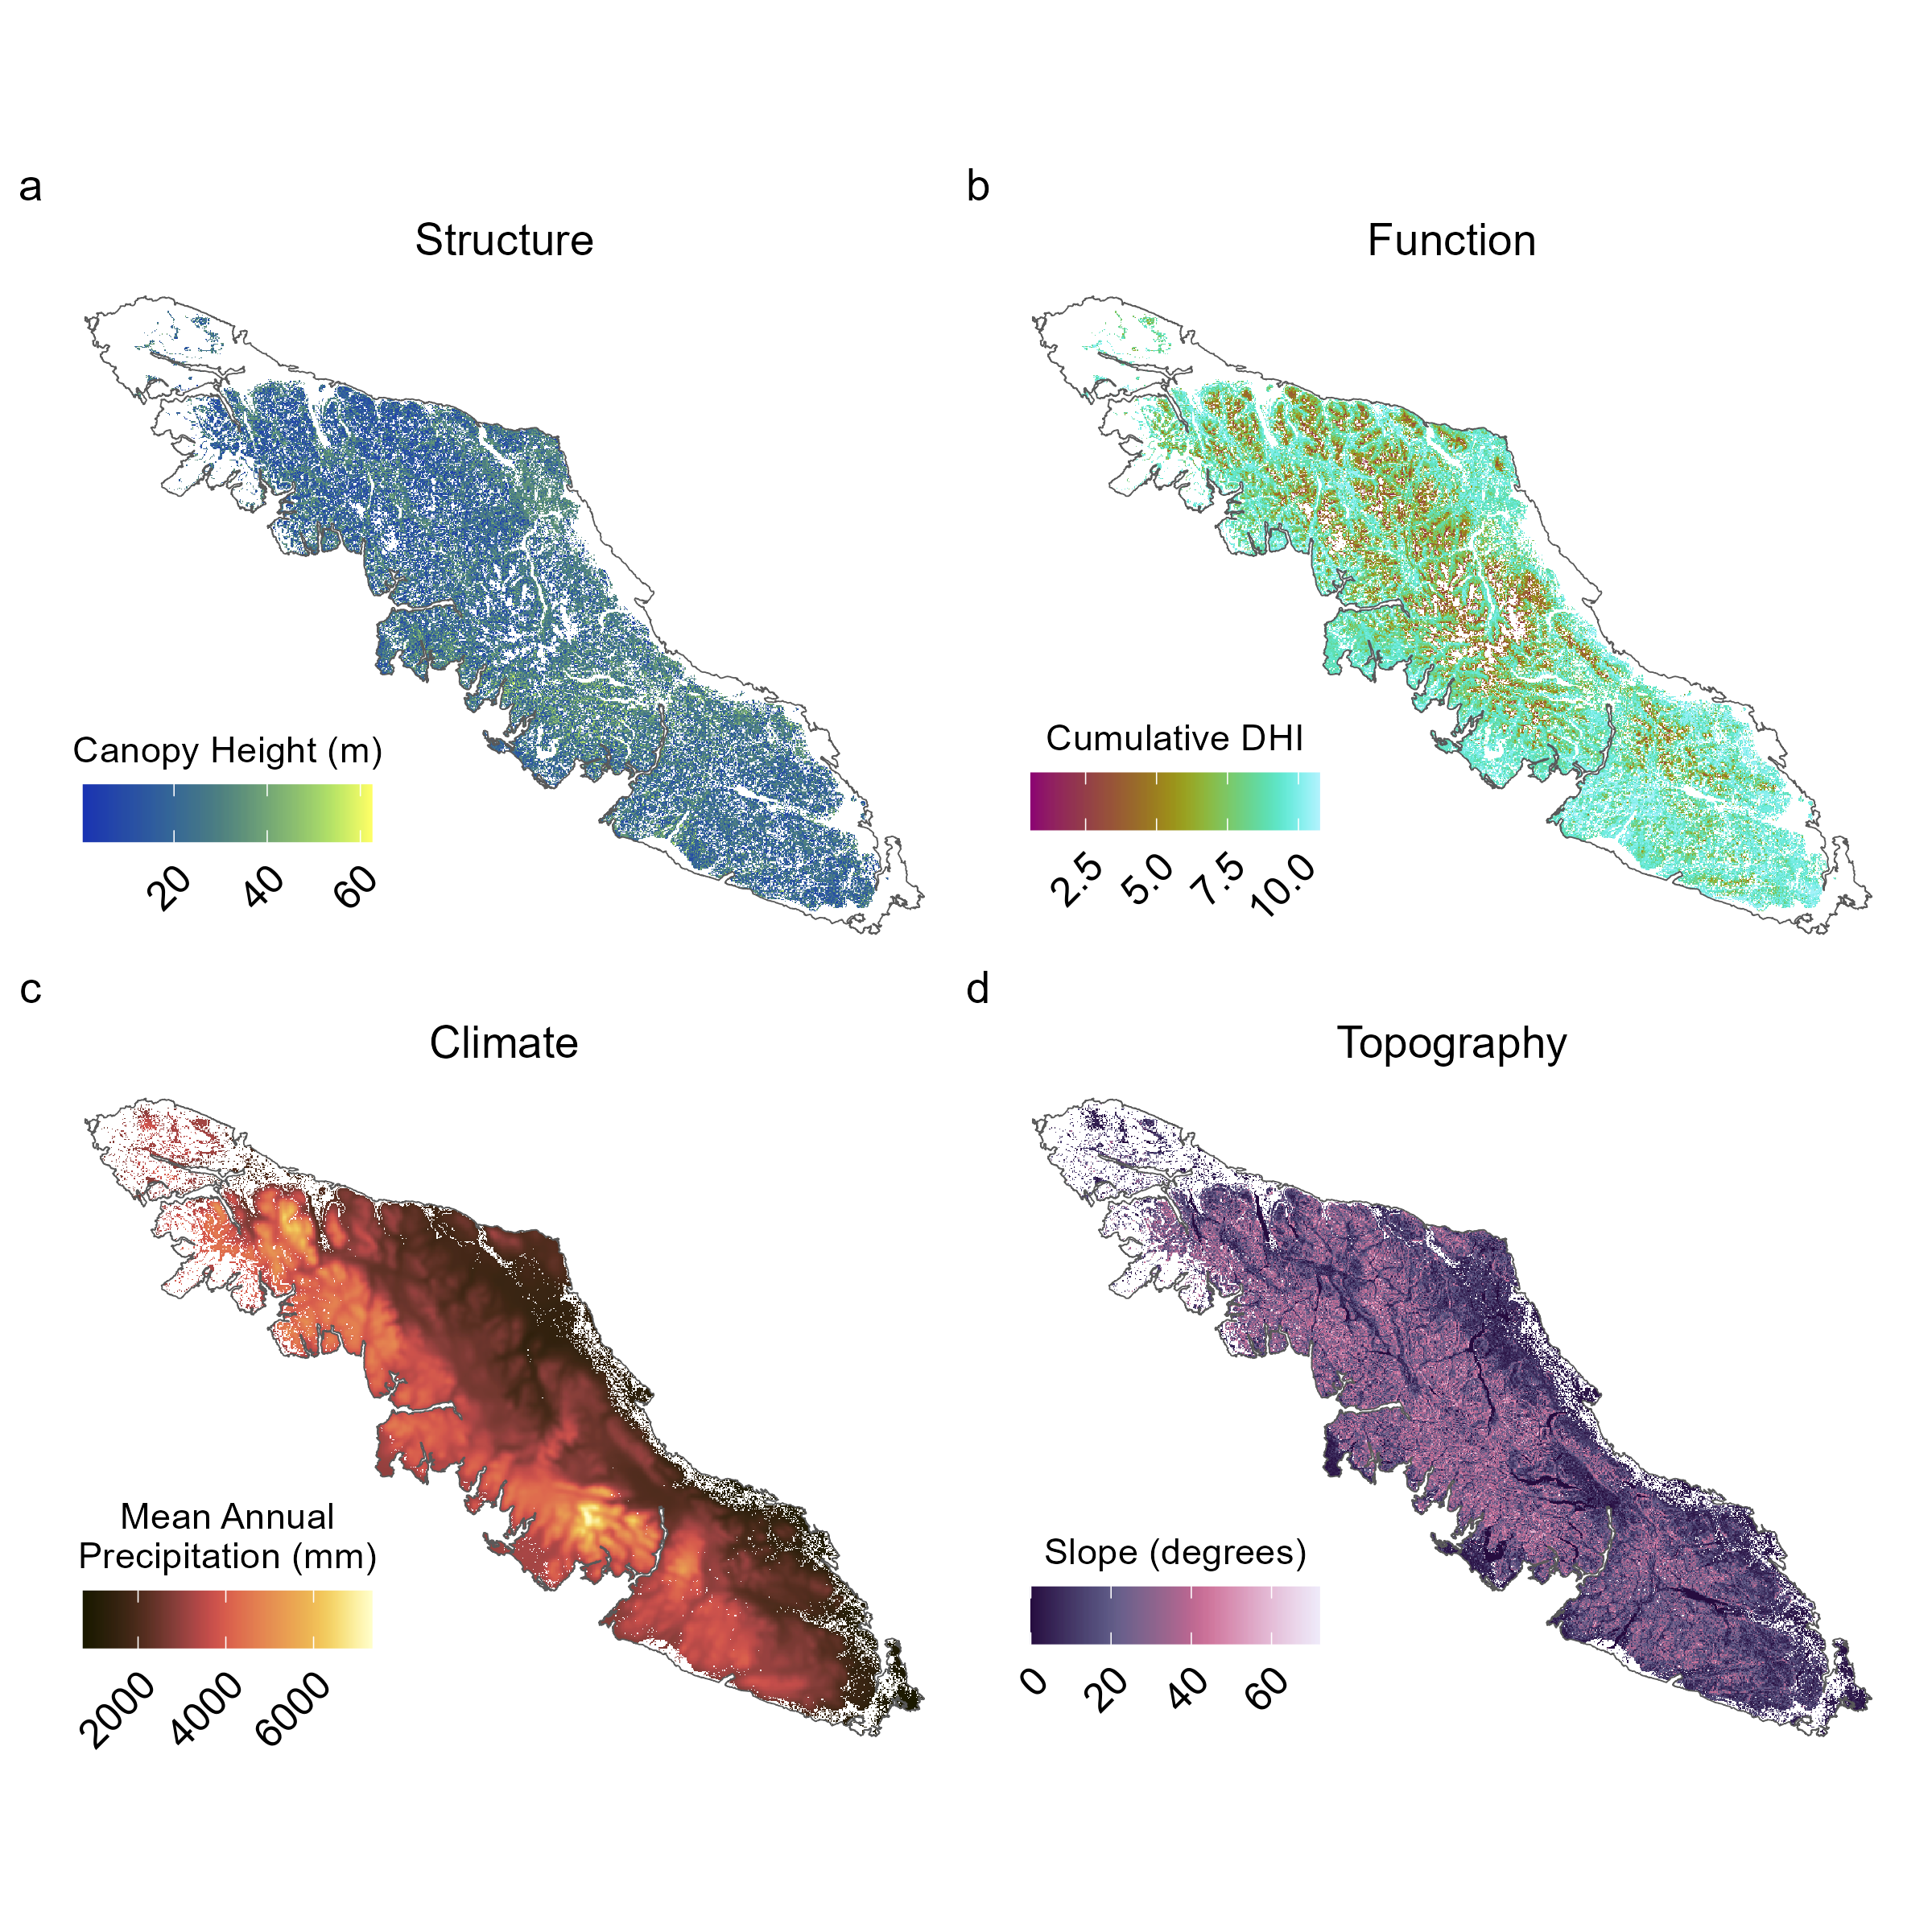
\includegraphics[width=8in,height=\textheight]{figures/data_figure.png}

}

\caption{\label{fig-data}Examples of each of the four major datasets
used in our study. Panels a and b show structure and function,
respectively, used for the calculation of sigma dissimilarity. Panels c
and d show climate and topography, respectively, used for the coarsened
exact matching procedure.}

\end{figure}%

\subsection{Calculating Ecological Dissimilarity}\label{sec-sim}

We calculated the sigma dissimilarity (Mahony et al., 2017) of forested
pixels across our study area by using an expanded coarsened exact
matching (CEM) technique (Iacus et al., 2012) (Figure~\ref{fig-flow})
for each forest type (broadleaf, coniferous, mixed wood, and
wetland-treed) (Hermosilla et al., 2018). The CEM technique creates
comparable groups of observations across covariates by initially
coarsening the covariates. In this instance, all six covariates
(elevation, slope, mean annual precipitation, mean annual temperature,
mean coldest month temperature, and mean warmest month temperature) were
coarsened into five quintiles, hereafter referred to as bins. CEM then
performs exact matching on the bins, with each pixel matched to a
climatically and topographically similar group of pixels within the
reference state (i.e.~Strathcona Park), hereafter referred to as
stratum. If inusfficient numbers of matched pixels were found in the
reference state, we calculated the stratum's nearest neighbour across
covariate bins, and sampled up to 100 pixels, while minimizing the
nearest neighbour distance. If the average nearest neighbour distance
was greater than two, that stratum was excluded from the analysis.

\phantomsection\label{cell-fig-flow}
\begin{figure}[H]

\centering{

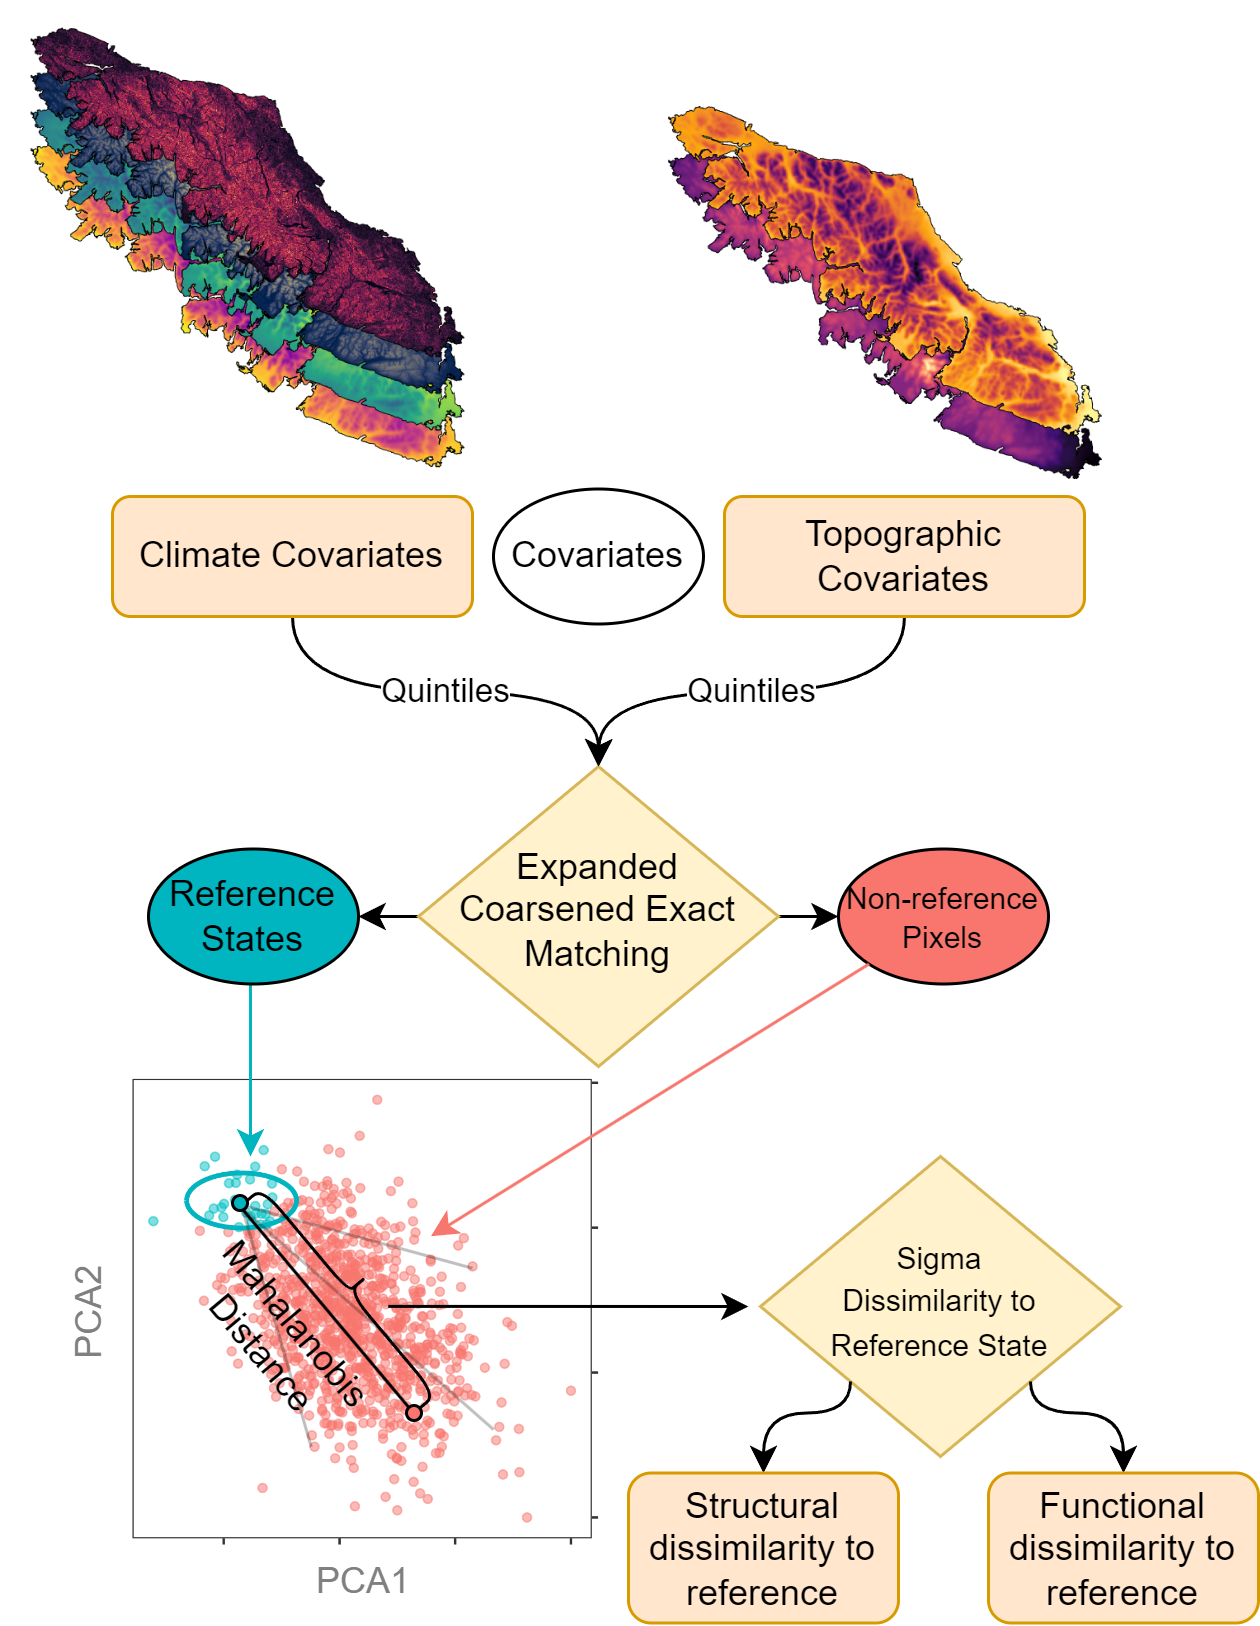
\includegraphics[width=4.2in,height=\textheight]{figures/flow.drawio.png}

}

\caption{\label{fig-flow}Conceptual flow diagram of the study.}

\end{figure}%

Following the matching procedure, we identified reference states as
undisturbed (human footprint = 0; no fire or harvesting disturbance)
(Hermosilla et al., 2015; Hirsh-Pearson et al., 2022) pixels by stratum
within Strathcona Park. We then determine the dissimilarity of all
pixels, in structural, functional, and structural + functional
attributes, to the reference states by calculating the sigma
dissimilarity metric. Sigma dissimilarity standardizes the Mahalanobian
distance (Mahalanobis, 1936) by rescaling it into percentiles of the chi
distribution to account for the effect of dimensionality when creating a
multivariate dissimilarity metric (Mahony et al., 2017). We calculated
sigma dissimilarity for every stratum with a suitable reference state as
generated by our matching procedure. This dissimilarity metric
effectively functions as a multivariate proxy for ecological integrity,
with higher values indicating a larger difference from near natural
conditions found within the reference state.

\subsection{Impacts of anthropogenic pressure on ecological
dissimilarity}\label{impacts-of-anthropogenic-pressure-on-ecological-dissimilarity}

To assess the cumulative impact of anthropogenic pressure on ecological
dissimilarity, we implement stratified sampling on all suitable stratum,
sampling 100 samples from each anthropogenic pressure class. For our
individual pressures, we sampled an additional 100 samples for each
pressure class. Sampling was performed using the \textbf{sgsR} (version
1.4.5) R package (Goodbody et al., 2023) with the Quiennec method
(Queinnec et al., 2021). Geospatial data processing was performed using
the \textbf{terra} (version 1.7-78) (Hijmans, 2024), \textbf{sf}
(version 1.0-16) (Pebesma, 2018; Pebesma and Bivand, 2023), and
\textbf{tidyterra} (version 0.6.1) (Hernangómez, 2023) R packages.

We used a one-way analysis of variance (ANOVA) with a critical p value
of 0.05 to identify statistically significant differences in the mean
similarity values across cumulative anthropogenic pressure classes. We
account for family-wise error rate in our ANOVAs using the
Holm-Bonferroni method (Holm, 1979), only continuing the analysis for
similarity variables with significant ANOVAs at the adjusted critical
value. We used a Tukey HSD post-hoc test to identify which means are
different from the control group (intact pixels), which also controls
for the family-wise error rate.

We follow the same protocol to identify the difference in means for each
anthropogenic pressure of interest (roads, population density, forestry,
and built environment). We compare each pressure to the same `no
pressure' values sampled in the cumulative pressure analysis. All
statistical analysis were conducted using the \textbf{rstatix} (version
0.7.2) R package (Kassambara, 2023).

\section{Results}\label{results}

We generated maps of sigma dissimilarity for ecosystem structure,
function, and structure + function across Vancouver Island as a measure
of ecological integrity (Figure~\ref{fig-regional}). We show three
representative examples within Vancouver Island to display the impact of
anthropogenic pressures on ecosystem similarity, displaying a region
near Lake Cowichan where harvesting is a common pressure
(Figure~\ref{fig-regional} A), a protected area (Elk Falls Provincial
Park) near Campbell River with high population density
(Figure~\ref{fig-regional} B), and a region with lower anthropogenic
pressures (Figure~\ref{fig-regional} C). Functional dissimilarity shows
higher variation across all three sites than functional or structural
and functional dissimilarity. The protected region near Campbell River
(Figure~\ref{fig-regional} B) has lower dissimilarity metrics for all
three metrics.

\phantomsection\label{cell-fig-regional}
\begin{figure}[H]

\centering{

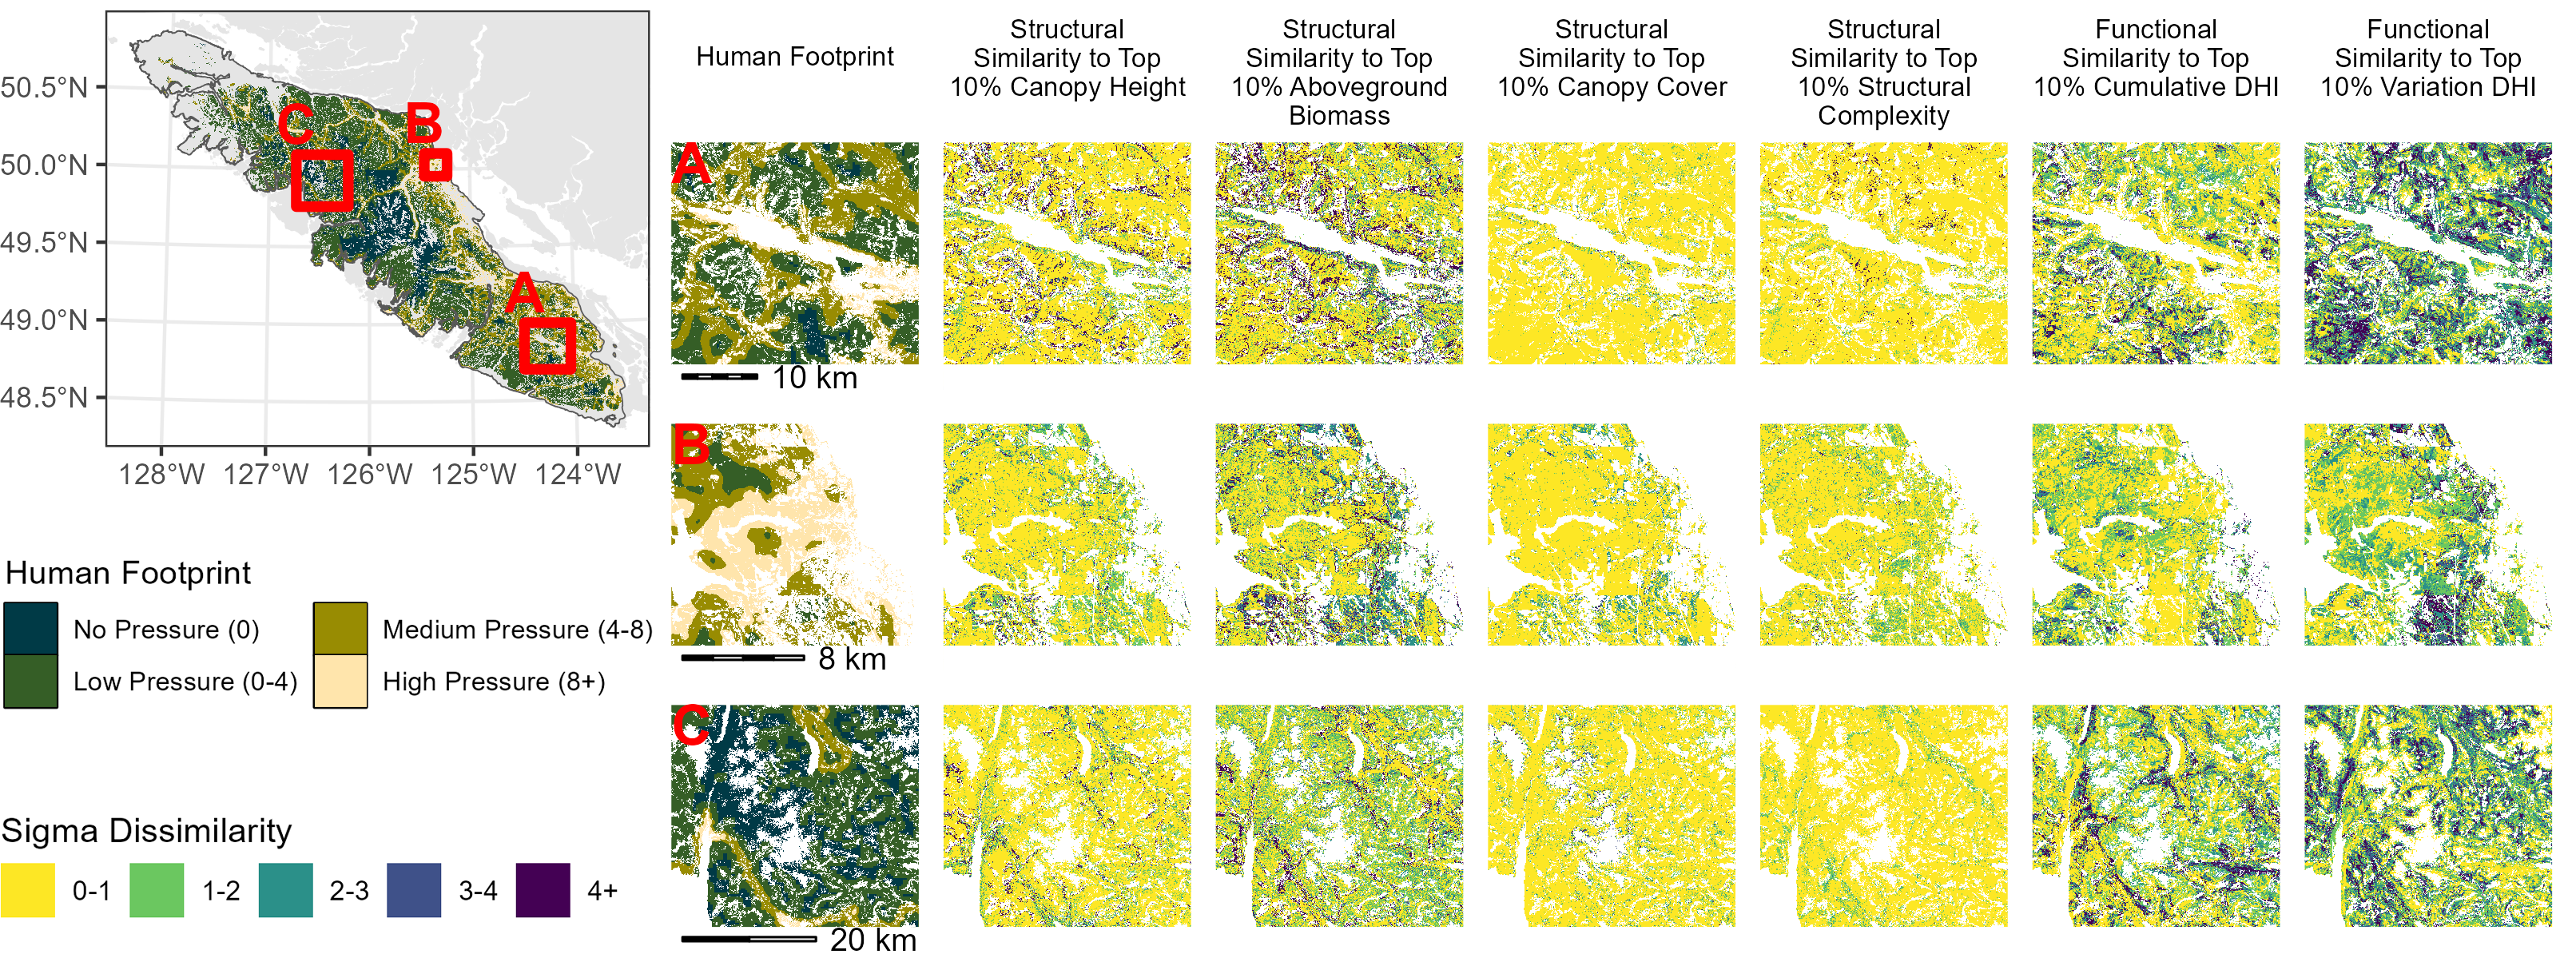
\includegraphics[width=10in,height=\textheight]{figures/multi_panel_inset_wide_PS.png}

}

\caption{\label{fig-regional}Regional details of the human footprint and
sigma dissimilarity across the sites on Vancouver Island. Subset A show
Cowichan Lake, a heavily harvested region. Subset B shows Elk Falls
Provincial Park, just outside Campbell River, a region with high
population density. Subset C shows a region with generally low
anthropogenic pressure.}

\end{figure}%

We used ANOVAs and post-hoc Tukey HSD tests to assess the influence of
the cumulative human footprint on ecological dissimilarity
(Figure~\ref{fig-boxplot-overall}) . Results indicate that structural
(ANOVA; p = 0.014) and structural + functional (ANOVA; p = 0.006)
dissimilarity was significantly different under varying anthropogenic
pressures. The functional dissimilarity metric did not significantly
vary with anthropogenic pressures. The Tukey HSD test revealed that high
levels of anthropogenic pressures significantly influence dissimilarity
to the structural (ANOVA; p \textless{} 0.01) and structural +
functional (ANOVA; p \textless{} 0.05) reference state. Medium and low
levels of anthropogenic pressures did not significantly influence any
dissimilarity metrics.

\phantomsection\label{cell-fig-boxplot-overall}
\begin{figure}[H]

\centering{

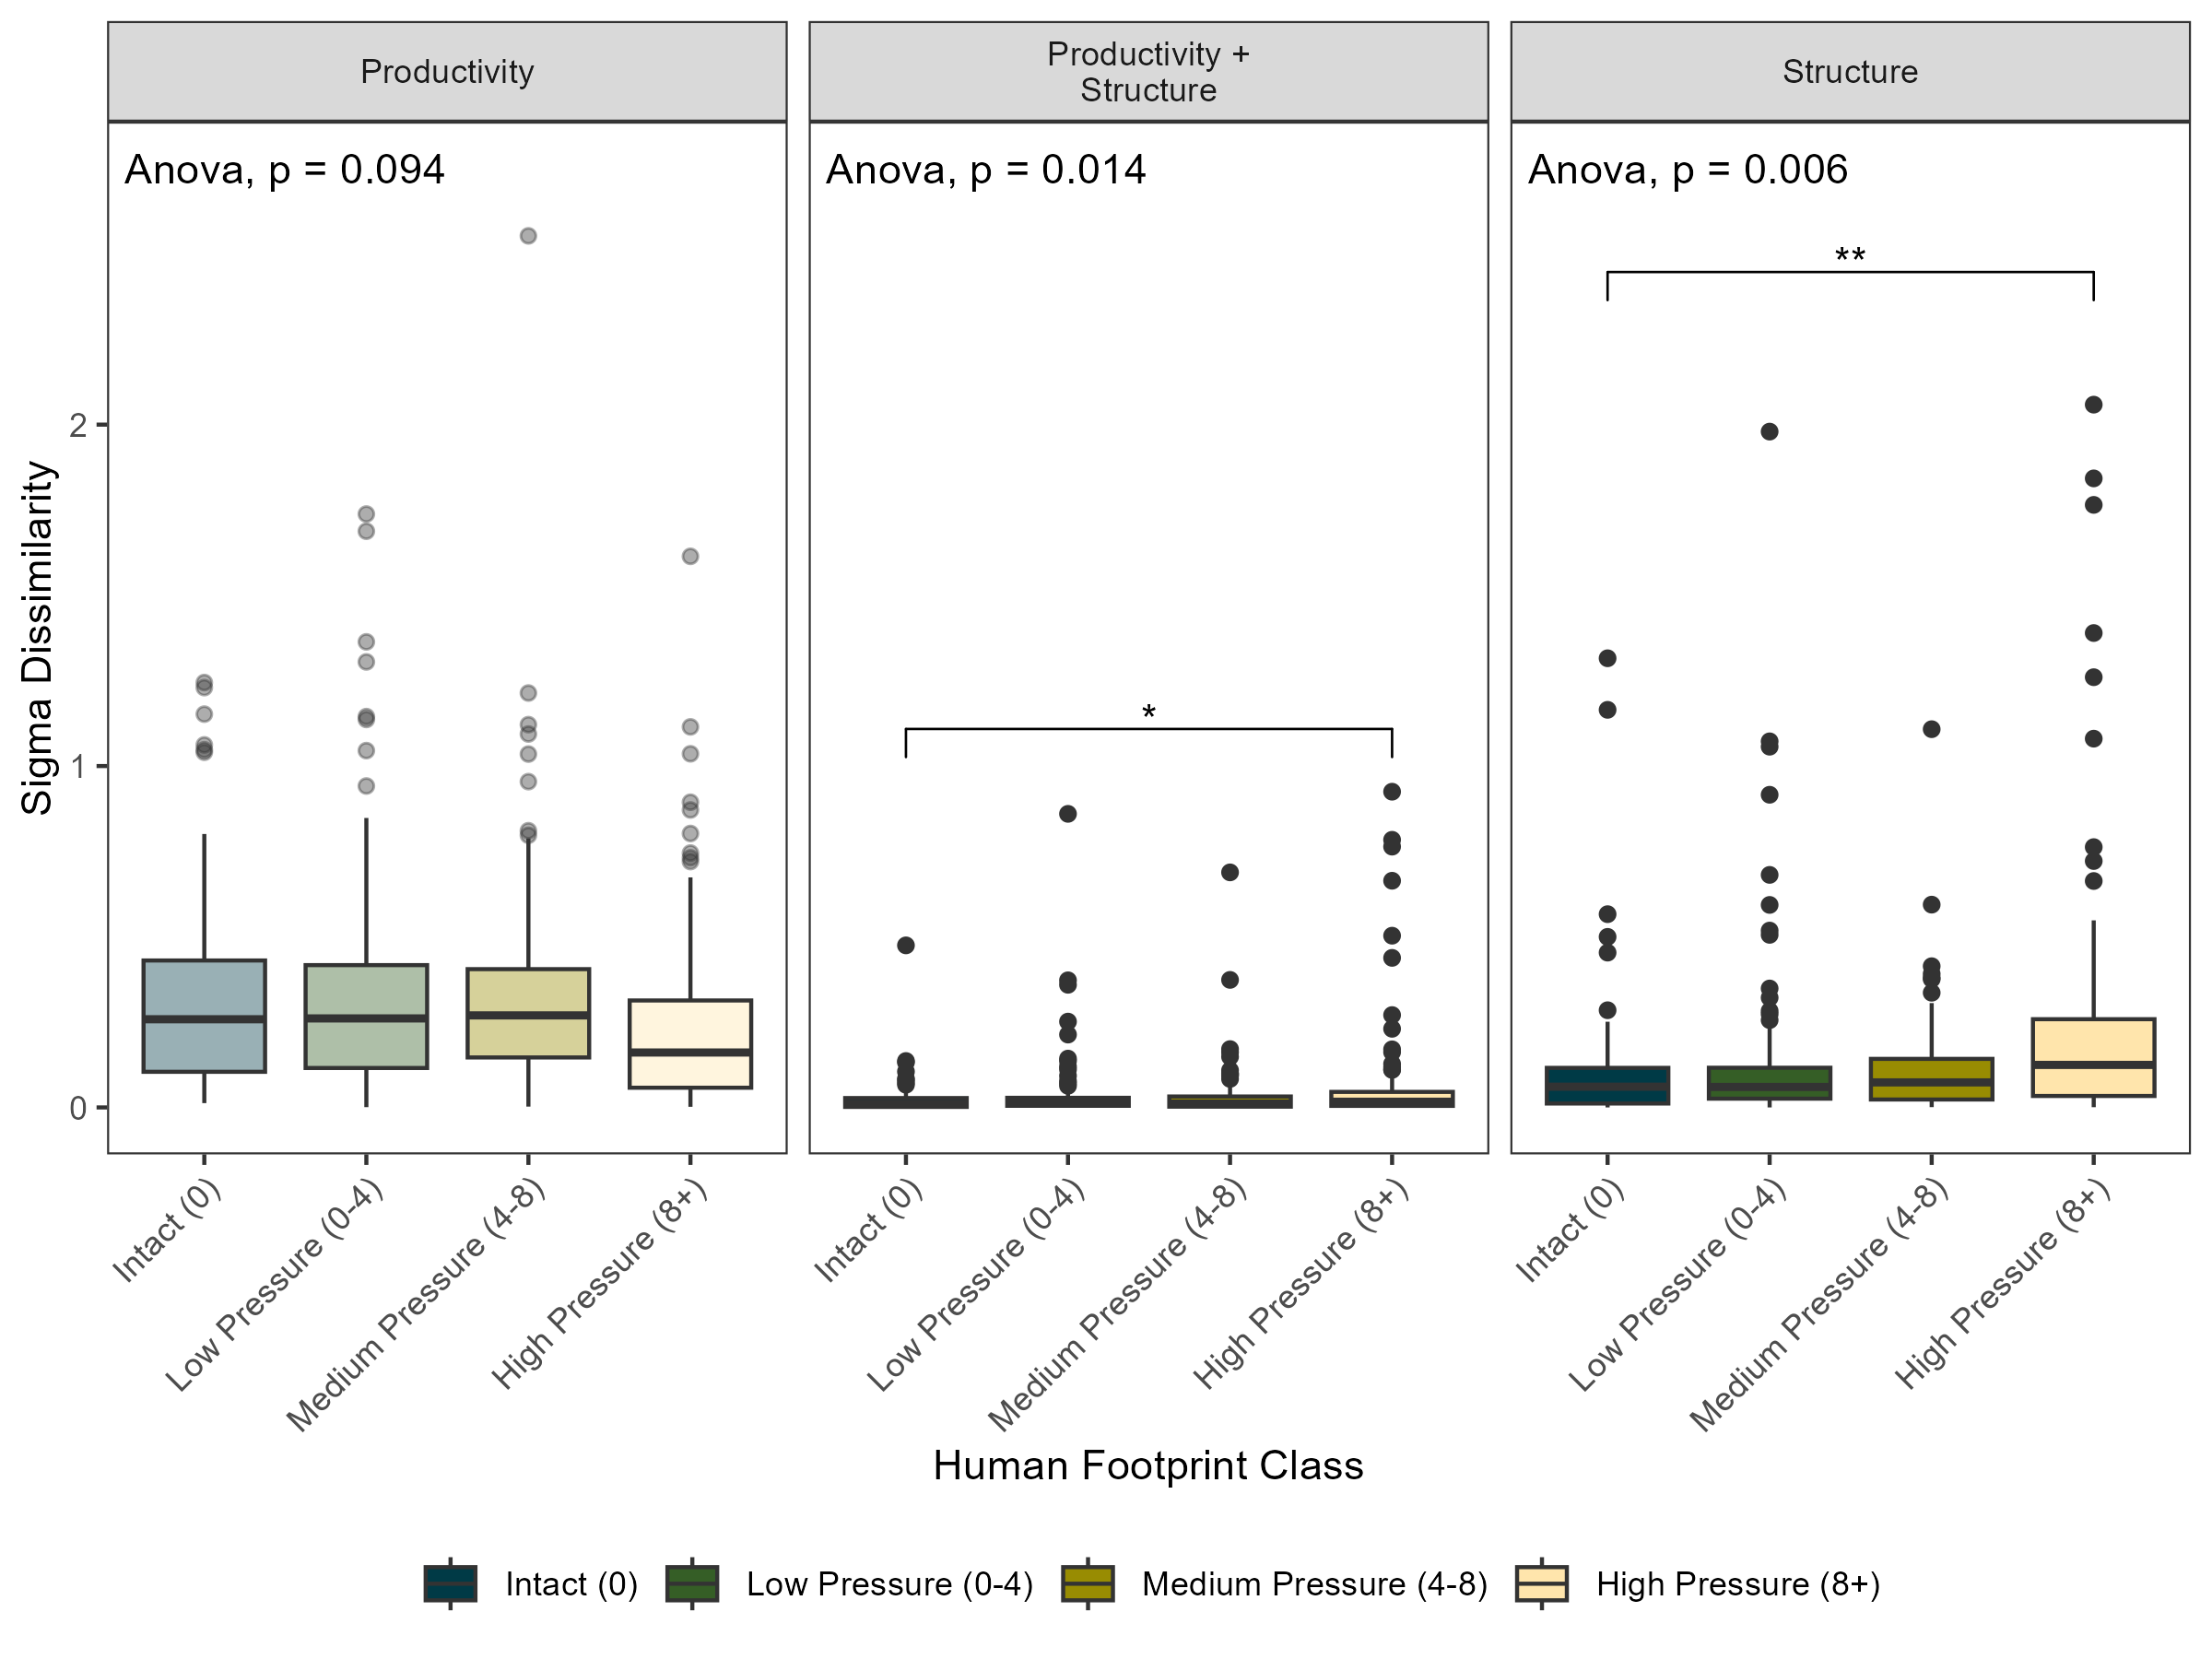
\includegraphics[width=8in,height=\textheight]{figures/mahal_boxplot_sig.png}

}

\caption{\label{fig-boxplot-overall}Boxplots of sigma similarity to the
reference state in Strathcona Provincial Park by cumulative human
footprint category. ANOVA p-values corrected using the Holm-Bonferroni
method. * indicates a Tukey HSD p-value \textless{} 0.05. ** indicates a
Tukey HSD p-value \textless{} 0.01.}

\end{figure}%

Further we assessed the impact of individual pressures on ecological
dissimilarity to the reference state
(Figure~\ref{fig-boxplot-individual}). We found that functional
dissimilarity was not significantly influenced by any anthropogenic
pressures, and that roads did not influence any type of ecological
dissimilarity (ANOVAs; all p \textgreater{} 0.05). Population density,
forestry and harvesting, and built environments did significantly
increase both structural and structural + functional dissimilarity
(ANOVAs; all p \textless{} 0.01). Only the highest levels of pressures
for each anthropogenic pressure category significantly influenced
ecological dissimilarity (ANOVAs; all p \textless{} 0.01).

\phantomsection\label{cell-fig-boxplot-individual}
\begin{figure}[H]

\centering{

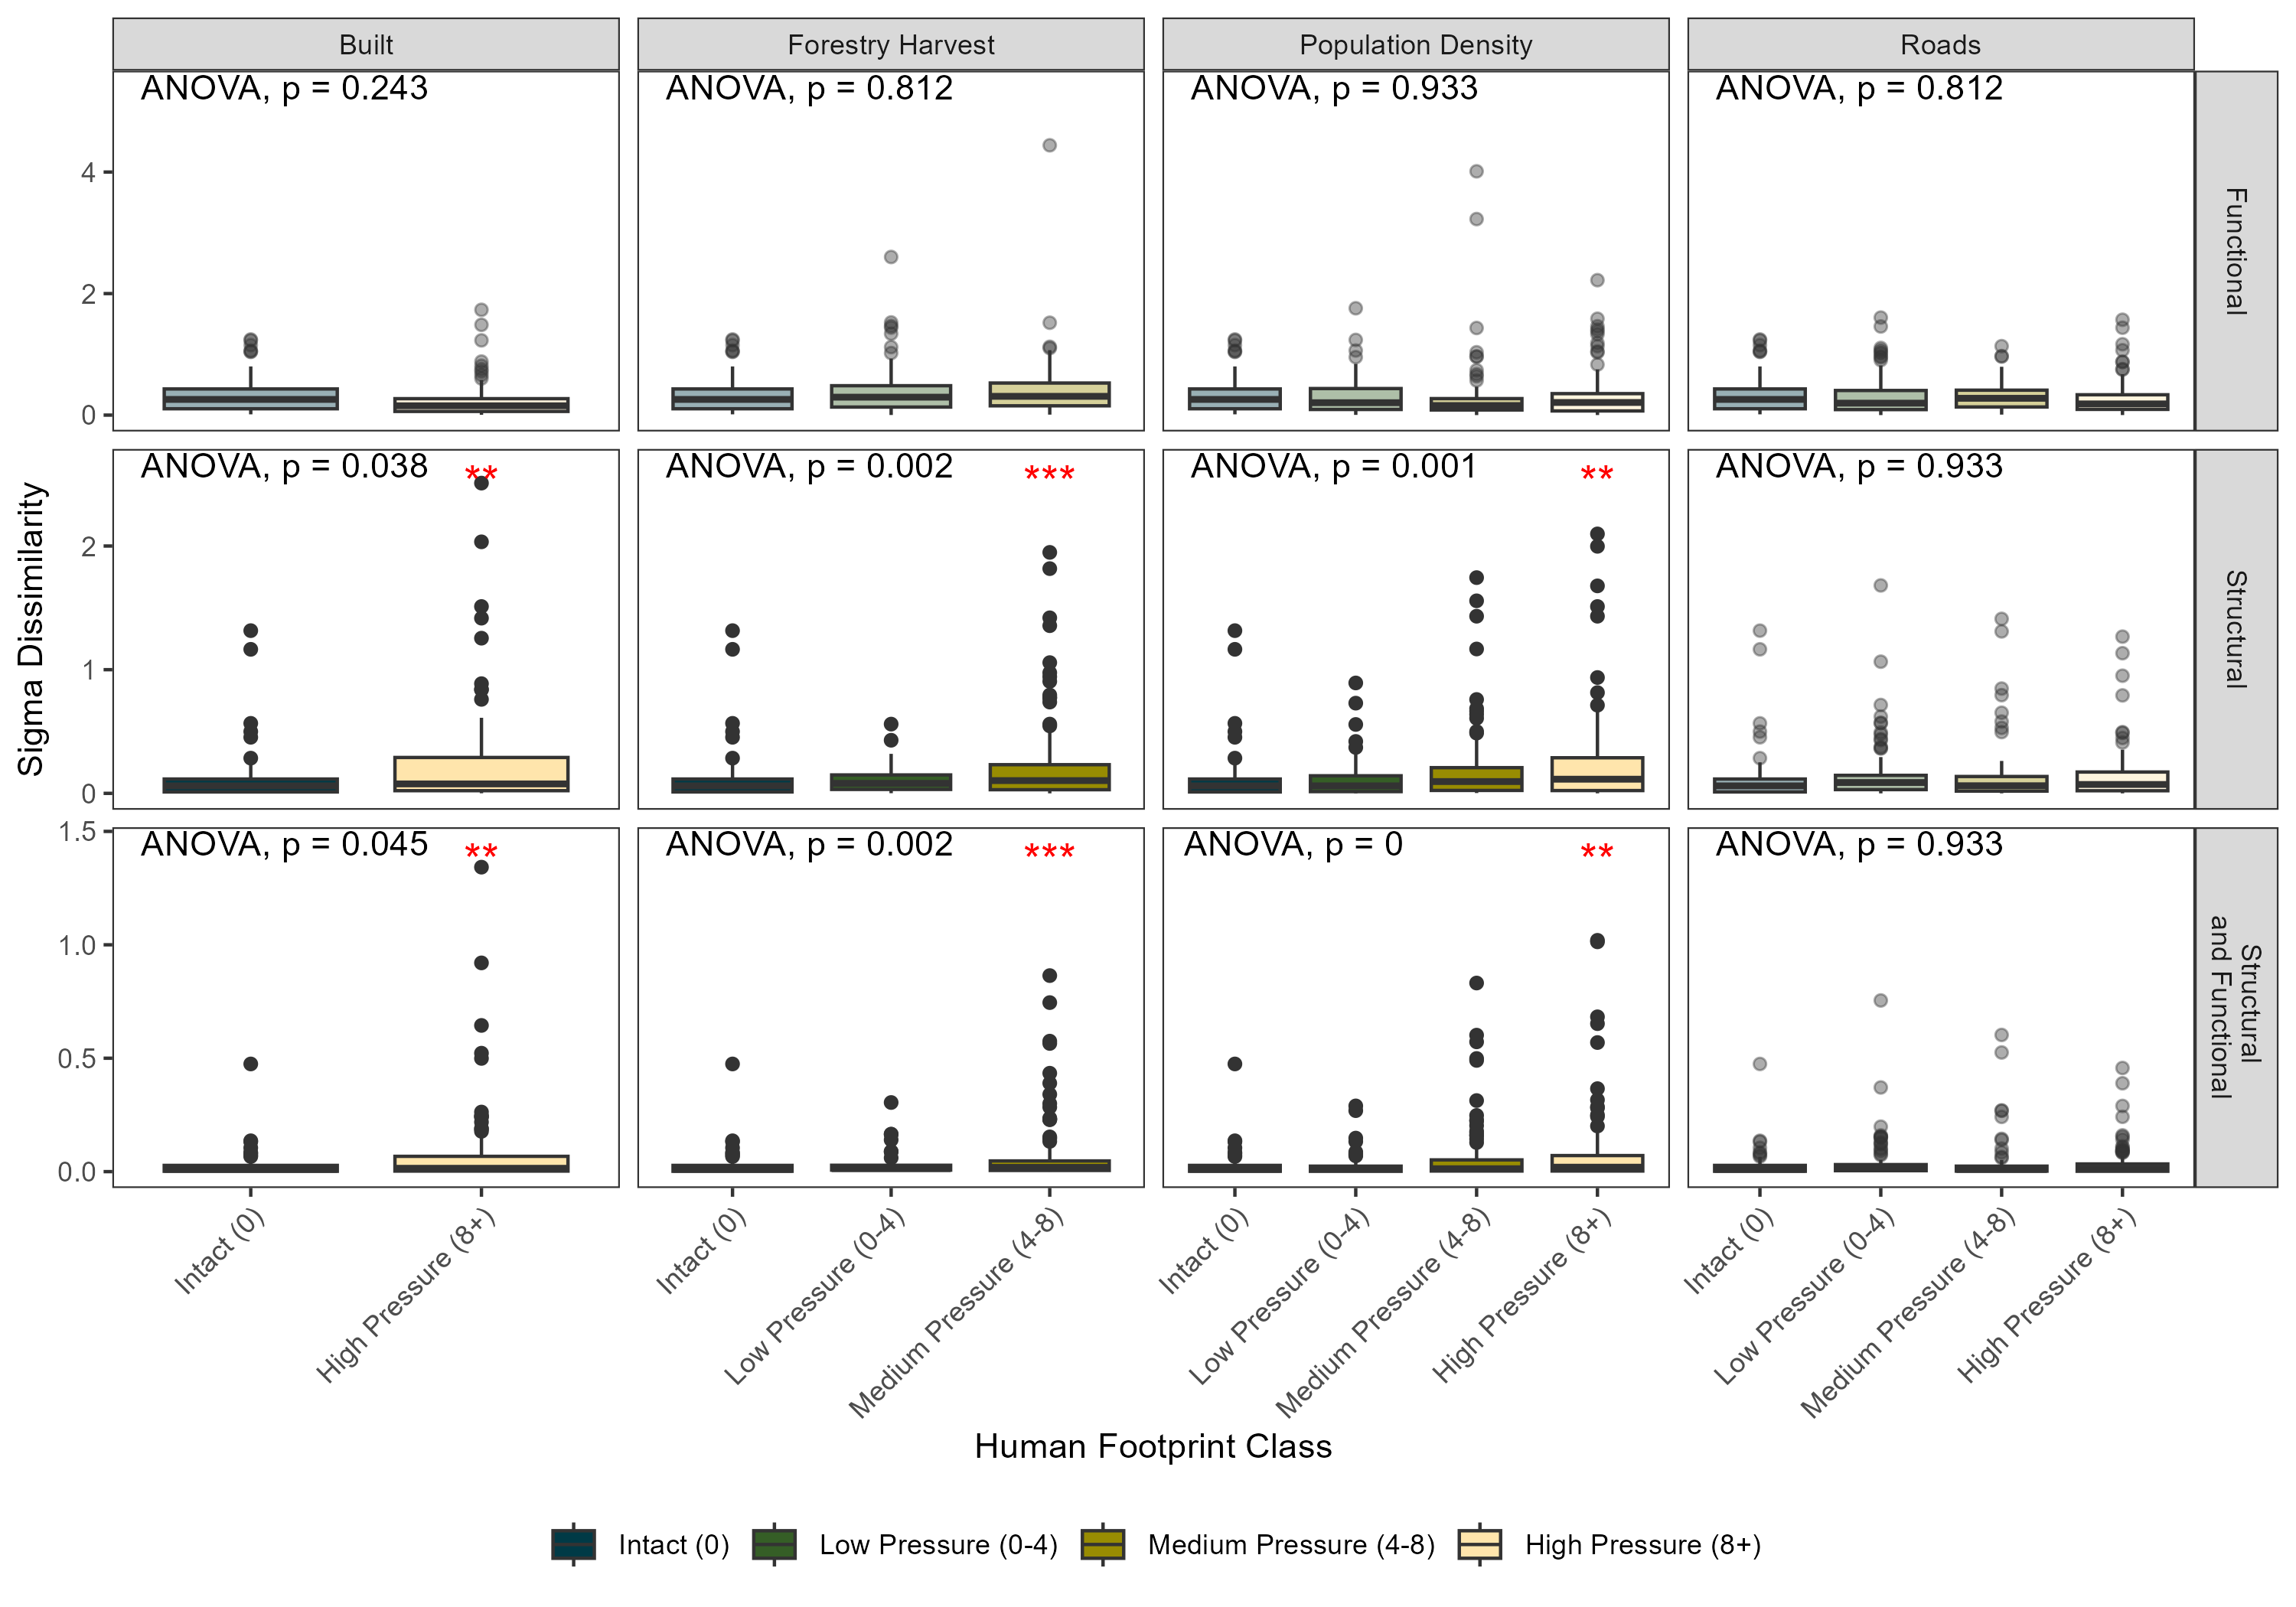
\includegraphics[width=10in,height=\textheight]{figures/indiv_boxplots.png}

}

\caption{\label{fig-boxplot-individual}Boxplots of sigma similarity to
the reference state in Strathcona Provincial Park by individual
anthropogenic pressures. ANOVA p-values corrected using the
Holm-Bonferroni method. ** indicates a Tukey HSD p-value \textless{}
0.01. *** indicates a Tukey HSD p-value \textless{} 0.001.}

\end{figure}%

\section{Discussion}\label{discussion}

Here, we propose a novel approach to assess ecological integrity across
forested ecosystems. Our method incorporates an expanded coarsened exact
matching technique (Iacus et al., 2012) and a multidimensional
dissimilarity metric (Mahony et al., 2017). This method integrates a
robust method for generating suitable reference states through the use
of a large, long-term protected area, and excluding any pressures and
disturbances, and estimates ecological integrity as dissimilarity to the
reference state by using the sigma dissimilarity metric, which accounts
for covariations in the data and varying dimensionality in input
datasets. The methodology is demonstrated on the forested areas of
Vancouver Island, which are environmentally similar to the reference
state, Strathcona Park. Furthermore, the influence of anthropogenic
pressure on ecological integrity is assessed. It was found that high
levels of anthropogenic pressure increase structural and structural +
functional dissimilarity, thus showing a reduction in ecological
integrity (Figure~\ref{fig-boxplot-overall};
Figure~\ref{fig-boxplot-individual}). However, functional dissimilarity
was never influenced by anthropogenic pressures.

Our structural dissimilarity metric is similar to other metrics of
forest condition, such as the forest structural condition index (Hansen
et al., 2019), however, it is not reliant on expert-set thresholds. This
potentially allows our metric to be transferable to new ecosystems and
environments, even allowing for the assessment of dissimilarity for
other ecosystems or a species' core ranges by changing the reference
state. This could be important for conservation efforts of rare and
threatened species. Further, we found that high cumulative anthropogenic
pressures increases structural dissimilarity
(Figure~\ref{fig-boxplot-overall}), and that high individual pressures,
except roads, also increase structural dissimilarty
(Figure~\ref{fig-boxplot-individual}). Prior research has generally
focused on tropical forests, where Bourgoin et al. (2024) found that
anthropogenic forest degradation influenced aboveground biomass and
canopy height, however, they focus on edge effects, fire, and selective
logging, rather than cumulative and individual anthropogenic pressures.
Li et al. (2023) also found a global impact of anthropogenic pressures
on forest structural density; however, they do not explore which facets
of anthropogenic pressure are the strongest driver of forest
degradation. Hansen et al. (2020) integrate forest structure and
anthropogenic pressure into the forest structural integrity index to
identify forest stands of high ecological value (high structural
quality; low anthropogenic footprint). We further this body of research
by assessing individual pressures on a multivariate metric of structural
similarity to a high-quality reference state
(Figure~\ref{fig-boxplot-individual}). While we assess impacts of
pressures on structural dissimilarity, integrating them together,
similar to Hansen et al. (2020), could help with protected area
prioritization efforts outside of moist tropical forests.

We also assess functional dissimilarity to high-integrity forests. We
found that functional dissimilarity more strongly varies than structural
dissimilarity (Figure~\ref{fig-regional}). However, we did not find any
significant influence of cumulative or individual anthropogenic
pressures on our forest functioning metrics
(Figure~\ref{fig-boxplot-overall}; Figure~\ref{fig-boxplot-individual}).
This may in part be due to the DHIs reliance on vegetation indices or
productivity estimates, in our case NDVI. Vegetation indices have been
shown to saturate at high levels of canopy cover and leaf area index
(Huete et al., 2002; Huete et al., 1997), which are common in our study
area. Recent research has shown that seasonality, here represented as
the Variation DHI, drives functional diversity in avian assemblages,
however, these results also strongly varied by region (Keyser et al.,
2024). It is possible that examining anthropogenic pressure impacts in
regions with more variation in canopy cover and stronger seasonality may
lead to differing results, as Vancouver Island has a moderate climate,
and is primarily dominated by conifer species Section~\ref{sec-study}.

We identified high-integrity forest reference states across a large
region using a data-driven approach. Often, it is common for suitable
reference states to be unavailable due to a lack of data on regions of
high ecological integrity, especially across large regions (McNellie et
al., 2020). We attempt to circumvent this by using a large,
long-established protected area (Strathcona Provincial Park;
Figure~\ref{fig-study}), and a matching technique that preserves
environmental similarity between reference states and their
counterparts. The long-established, large protected area ensures that
little anthropogenic pressures or modification have been made to the
landscape, while also guaranteeing that the reference state is
attainable for a given topography and climate (Corlett, 2016; Hobbs et
al., 2014) due to contemporary nature of the reference state. Our
matching technique (coarsened exact matching, combined with a nearest
neighbour approach when no exact match is available) allows us to
generate reference states in a near wall-to-wall fashion, which ensures
environmental consistency between reference state and compared pixels.

Our techniques move beyond traditional impact evaluation techniques
(Ferraro, 2009) commonly used in protected area effectiveness
assessments by generating spatially explicit maps of ecological
dissimilarity, and generating a multivariate, rather than univariate,
assessment of similarity to high ecological integrity forests. While our
methods use a data-driven approach to derive reference states using a
high-quality protected area, the method is inherently reference state
agnostic. Dissimilarity metrics could be generated for a specific
ecosystem, species, or community at landscape scales, identifying areas
with similar structural and functional conditions. This could be
especially relevant for species with known habitat requirements, such as
the marbled murrelet (\emph{Brachyramphus marmoratus}) needing tall,
complex forests as nesting habitat (Cosgrove et al., 2024)

Assessing individual pressure influences on the environment is also
relevant to questions of how cumulative anthropogenic pressure maps are
calculated. There is an ongoing debate surrounding anthropogenic
pressure mapping methods, as there is little information on mechanistic
interactions between pressures (Arias-Patino et al., 2024). We assess
individual pressures on ecological dissimilarity in forests across
Vancouver Island, Canada, an advancement upon the current standard of
using a single value of cumulative anthropogenic pressure (Bourgoin et
al., 2024; Li et al., 2023). Similar methods could be used to examine
mechanistic pressure interactions across large scales by examining
combinations of pressures rather than individual or overall impacts.

\section{Conclusion}\label{conclusion}

Identifying the location of high-integrity forests is integral to
conservation efforts, especially when considering protected area
management (Hansen et al., 2021; Pillay et al., 2024a). Until recently,
area based conservation has dominated management strategies, which does
not ensure that high-integrity ecosystems, typically having high
biodiversity and ecosystem services present, are protected (Ferrier et
al., 2024; Pillay et al., 2024a). Recent efforts to identify
high-integrity forests have been primarily focused on moist tropical
forests (Hansen et al., 2019), which contain large numbers of threatened
species reliant on intact forest structures (Pillay et al., 2024b). Due
to their focus on moist tropical forests, their methodology cannot
easily be transferred to other forested ecosystems, particularly due to
their focus on tall, complex trees (Hansen et al., 2019) without
considering local environmental conditions. Here, we use matching
techniques to circumvent this, and use sigma dissimilarity to consider
additional structural and functional information, allowing us to
identify high-integrity forests without relying on expert defined
thresholds which may not be suitable or available in all biomes. This
advance can be used to conservation planning strategies, as we work
towards the 30x30 goal outlined in the GBF (Convention on Biological
Diversity, 2023).

\section{Acknowledgements}\label{acknowledgements}

This research was funded by NSERC support of Coops (RGPIN-2024-04402).
Remote sensing data products used in this research are free and open and
available for download at \url{https://ca.nfis.org/maps_eng.html}. The
authors thank Dr.~Michael A. Wulder and Dr.~Joanne C. White for
development and early access to these National Terrestrial Ecosystem
Mapping System (NTEMS) products. They thank Dr.~Elena Razenkova for
early access to the Landsat-derived Dynamic Habitat Indices. ERM would
like to thank the members of the IRSS for many helpful conversations
throughout the preparation of this manuscript.

\section{Ethics}\label{ethics}

The authors declare no conflicts of interest.

\newpage

\section*{References}\label{references}
\addcontentsline{toc}{section}{References}

\phantomsection\label{refs}
\begin{CSLReferences}{1}{0}
\vspace{1em}

\bibitem[\citeproctext]{ref-abrams2020}
Abrams, M., Crippen, R., Fujisada, H., 2020. ASTER Global Digital
Elevation Model (GDEM) and ASTER Global Water Body Dataset (ASTWBD).
Remote Sensing 12, 1156. \url{https://doi.org/10.3390/rs12071156}

\bibitem[\citeproctext]{ref-ali2019}
Ali, A., 2019. Forest stand structure and functioning: Current knowledge
and future challenges. Ecological Indicators 98, 665--677.
\url{https://doi.org/10.1016/j.ecolind.2018.11.017}

\bibitem[\citeproctext]{ref-andrew2024}
Andrew, M.E., Bolton, D.K., Rickbeil, G.J.M., Coops, N.C., 2024. Facets
of functional diversity support niche-based explanations for Australian
biodiversity gradients. Journal of Biogeography 51, 467--482.
\url{https://doi.org/10.1111/jbi.14770}

\bibitem[\citeproctext]{ref-andrew2012a}
Andrew, M.E., Wulder, M.A., Coops, N.C., Baillargeon, G., 2012.
Beta-diversity gradients of butterflies along productivity axes. Global
Ecology and Biogeography 21, 352--364.
\url{https://doi.org/10.1111/j.1466-8238.2011.00676.x}

\bibitem[\citeproctext]{ref-arcese1997}
Arcese, P., Sinclair, A.R.E., 1997. The role of protected areas as
ecological baselines. The Journal of Wildlife Management 61, 587--602.
\url{https://doi.org/10.2307/3802167}

\bibitem[\citeproctext]{ref-arias-patino2024}
Arias-Patino, M., Johnson, C.J., Schuster, R., Wheate, R.D., Venter, O.,
2024. Accuracy, uncertainty, and biases in cumulative pressure mapping.
Ecological Indicators 166, 112407.
\url{https://doi.org/10.1016/j.ecolind.2024.112407}

\bibitem[\citeproctext]{ref-bergen2009}
Bergen, K.M., Goetz, S.J., Dubayah, R.O., Henebry, G.M., Hunsaker, C.T.,
Imhoff, M.L., Nelson, R.F., Parker, G.G., Radeloff, V.C., 2009. Remote
sensing of vegetation 3-d structure for biodiversity and habitat: Review
and implications for lidar and radar spaceborne missions. Journal of
Geophysical Research-Biogeosciences 114, G00E06.
\url{https://doi.org/10.1029/2008JG000883}

\bibitem[\citeproctext]{ref-berry2007}
Berry, S., Mackey, B., Brown, T., 2007. Potential applications of
remotely sensed vegetation greenness to habitat analysis and the
conservation of dispersive fauna. Pacific Conservation Biology 13,
120--127. \url{https://doi.org/10.1071/PC070120}

\bibitem[\citeproctext]{ref-bourgoin2024}
Bourgoin, C., Ceccherini, G., Girardello, M., Vancutsem, C., Avitabile,
V., Beck, P.S.A., Beuchle, R., Blanc, L., Duveiller, G., Migliavacca,
M., Vieilledent, G., Cescatti, A., Achard, F., 2024. Human degradation
of tropical moist forests is greater than previously estimated. Nature
631, 570--576. \url{https://doi.org/10.1038/s41586-024-07629-0}

\bibitem[\citeproctext]{ref-burns1990}
Burns, R.M., 1990. Silvics of North America. U.S. Department of
Agriculture, Forest Service.

\bibitem[\citeproctext]{ref-cardinale2012}
Cardinale, B.J., Duffy, J.E., Gonzalez, A., Hooper, D.U., Perrings, C.,
Venail, P., Narwani, A., Mace, G.M., Tilman, D., Wardle, D.A., Kinzig,
A.P., Daily, G.C., Loreau, M., Grace, J.B., Larigauderie, A.,
Srivastava, D.S., Naeem, S., 2012. Biodiversity loss and its impact on
humanity. Nature 486, 59--67. \url{https://doi.org/10.1038/nature11148}

\bibitem[\citeproctext]{ref-reporto2023}
Convention on Biological Diversity, 2023. Report of the conference of
the parties to the {Convention} on {Biological Diversity} on the second
part of its fifteenth meeting (No. CBD/COP/15/17).

\bibitem[\citeproctext]{ref-coops2019}
Coops, N.C., Bolton, D.K., Hobi, M.L., Radeloff, V.C., 2019. Untangling
multiple species richness hypothesis globally using remote sensing
habitat indices. Ecological Indicators 107.
\url{https://doi.org/10.1016/j.ecolind.2019.105567}

\bibitem[\citeproctext]{ref-WOS:000265076300011}
Coops, N.C., Waring, R.H., Wulder, M.A., Pidgeon, A.M., Radeloff, V.C.,
2009a. Bird diversity: A predictable function of satellite-derived
estimates of seasonal variation in canopy light absorbance across the
{United States}. Journal of Biogeography 36, 905--918.
\url{https://doi.org/10.1111/j.1365-2699.2008.02053.x}

\bibitem[\citeproctext]{ref-coops2009ecoinfo}
Coops, N.C., Wulder, M.A., Iwanicka, D., 2009b. Demonstration of a
satellite-based index to monitor habitat at continental-scales.
Ecological Informatics 9, 948--958.
\url{https://doi.org/10.1016/j.ecolind.2008.11.003}

\bibitem[\citeproctext]{ref-corlett2016}
Corlett, R.T., 2016. Restoration, reintroduction, and rewilding in a
changing world. Trends in Ecology \& Evolution 31, 453--462.
\url{https://doi.org/10.1016/j.tree.2016.02.017}

\bibitem[\citeproctext]{ref-cosgrove2024}
Cosgrove, C.F., Coops, N.C., Waterhouse, F.L., Goodbody, T.R.H., 2024.
Modeling marbled murrelet nesting habitat: A quantitative approach using
airborne laser scanning data in british columbia, canada. Avian
Conservation and Ecology 19.
\url{https://doi.org/10.5751/ACE-02585-190105}

\bibitem[\citeproctext]{ref-daniels2006}
Daniels, L.D., Gray, R.W., 2006. Disturbance regimes in coastal British
Columbia. Journal of Ecosystems and Management 7.
\url{https://doi.org/10.22230/jem.2006v7n2a542}

\bibitem[\citeproctext]{ref-duncanson2023}
Duncanson, L., Liang, M., Leitold, V., Armston, J., Krishna Moorthy,
S.M., Dubayah, R., Costedoat, S., Enquist, B.J., Fatoyinbo, L., Goetz,
S.J., Gonzalez-Roglich, M., Merow, C., Roehrdanz, P.R., Tabor, K.,
Zvoleff, A., 2023. The effectiveness of global protected areas for
climate change mitigation. Nature Communications 14, 2908.
\url{https://doi.org/10.1038/s41467-023-38073-9}

\bibitem[\citeproctext]{ref-ferraro2009}
Ferraro, P.J., 2009. Counterfactual thinking and impact evaluation in
environmental policy. New Directions for Evaluation 2009, 75--84.
\url{https://doi.org/10.1002/ev.297}

\bibitem[\citeproctext]{ref-ferrier2024}
Ferrier, S., Ware, C., Austin, J.M., Grantham, H.S., Harwood, T.D.,
Watson, J.E.M., 2024. Ecosystem extent is a necessary but not sufficient
indicator of the state of global forest biodiversity. Conservation
Letters 17, e13045. \url{https://doi.org/10.1111/conl.13045}

\bibitem[\citeproctext]{ref-gao2014}
Gao, T., Hedblom, M., Emilsson, T., Nielsen, A.B., 2014. The role of
forest stand structure as biodiversity indicator. Forest Ecology and
Management 330, 82--93.
\url{https://doi.org/10.1016/j.foreco.2014.07.007}

\bibitem[\citeproctext]{ref-geldmann2019}
Geldmann, J., Manica, A., Burgess, N.D., Coad, L., Balmford, A., 2019. A
global-level assessment of the effectiveness of protected areas at
resisting anthropogenic pressures. Proceedings of the National Academy
of Sciences 116, 23209--23215.
\url{https://doi.org/10.1073/pnas.1908221116}

\bibitem[\citeproctext]{ref-goodbody2023}
Goodbody, T.R.H., Coops, N.C., Queinnec, M., White, J.C., Tompalski, P.,
Hudak, A.T., Auty, D., Valbuena, R., LeBoeuf, A., Sinclair, I.,
McCartney, G., Prieur, J.-F., Woods, M.E., 2023. sgsR: A structurally
guided sampling toolbox for LiDAR-based forest inventories. Forestry: An
International Journal of Forest Research 96, 411--424.
\url{https://doi.org/10.1093/forestry/cpac055}

\bibitem[\citeproctext]{ref-gorelick2017}
Gorelick, N., Hancher, M., Dixon, M., Ilyushchenko, S., Thau, D., Moore,
R., 2017. Google Earth Engine: Planetary-scale geospatial analysis for
everyone. Remote Sensing of Environment, Big Remotely Sensed Data:
tools, applications and experiences 202, 18--27.
\url{https://doi.org/10.1016/j.rse.2017.06.031}

\bibitem[\citeproctext]{ref-grantham2020}
Grantham, H.S., Duncan, A., Evans, T.D., Jones, K.R., Beyer, H.L.,
Schuster, R., Walston, J., Ray, J.C., Robinson, J.G., Callow, M.,
Clements, T., Costa, H.M., DeGemmis, A., Elsen, P.R., Ervin, J., Franco,
P., Goldman, E., Goetz, S., Hansen, A., Hofsvang, E., Jantz, P.,
Jupiter, S., Kang, A., Langhammer, P., Laurance, W.F., Lieberman, S.,
Linkie, M., Malhi, Y., Maxwell, S., Mendez, M., Mittermeier, R., Murray,
N.J., Possingham, H., Radachowsky, J., Saatchi, S., Samper, C.,
Silverman, J., Shapiro, A., Strassburg, B., Stevens, T., Stokes, E.,
Taylor, R., Tear, T., Tizard, R., Venter, O., Visconti, P., Wang, S.,
Watson, J.E.M., 2020. Anthropogenic modification of forests means only
40. Nature Communications 11, 5978.
\url{https://doi.org/10.1038/s41467-020-19493-3}

\bibitem[\citeproctext]{ref-guo2017}
Guo, X., Coops, N.C., Tompalski, P., Nielsen, S.E., Bater, C.W., John
Stadt, J., 2017. Regional mapping of vegetation structure for
biodiversity monitoring using airborne lidar data. Ecological
Informatics 38, 50--61.
\url{https://doi.org/10.1016/j.ecoinf.2017.01.005}

\bibitem[\citeproctext]{ref-hansen2019}
Hansen, A., Barnett, K., Jantz, P., Phillips, L., Goetz, S.J., Hansen,
M., Venter, O., Watson, J.E.M., Burns, P., Atkinson, S.,
Rodríguez-Buritica, S., Ervin, J., Virnig, A., Supples, C., De Camargo,
R., 2019. Global humid tropics forest structural condition and forest
structural integrity maps. Scientific Data 6, 232.
\url{https://doi.org/10.1038/s41597-019-0214-3}

\bibitem[\citeproctext]{ref-hansen2020}
Hansen, A.J., Burns, P., Ervin, J., Goetz, S.J., Hansen, M., Venter, O.,
Watson, J.E.M., Jantz, P.A., Virnig, A.L.S., Barnett, K., Pillay, R.,
Atkinson, S., Supples, C., Rodríguez-Buritica, S., Armenteras, D., 2020.
A policy-driven framework for conserving the best of Earth{'}s remaining
moist tropical forests. Nature Ecology \& Evolution 4, 1377--1384.
\url{https://doi.org/10.1038/s41559-020-1274-7}

\bibitem[\citeproctext]{ref-hansen2021}
Hansen, A.J., Noble, B.P., Veneros, J., East, A., Goetz, S.J., Supples,
C., Watson, J.E.M., Jantz, P.A., Pillay, R., Jetz, W., Ferrier, S.,
Grantham, H.S., Evans, T.D., Ervin, J., Venter, O., Virnig, A.L.S.,
2021. Toward monitoring forest ecosystem integrity within the post-2020
Global Biodiversity Framework. Conservation Letters 14, e12822.
\url{https://doi.org/10.1111/conl.12822}

\bibitem[\citeproctext]{ref-hermosilla2018}
Hermosilla, T., Wulder, M.A., White, J.C., Coops, N.C., Hobart, G.W.,
2018. Disturbance-informed annual land cover classification maps of
canada's forested ecosystems for a 29-year landsat time series. Canadian
Journal of Remote Sensing 44, 6787.
\url{https://doi.org/10.1080/07038992.2018.1437719}

\bibitem[\citeproctext]{ref-hermosilla2015}
Hermosilla, T., Wulder, M.A., White, J.C., Coops, N.C., Hobart, G.W.,
2015. An integrated landsat time series protocol for change detection
and generation of annual gap-free surface reflectance composites. Remote
Sensing of Environment 158, 220234.
\url{https://doi.org/10.1016/j.rse.2014.11.005}

\bibitem[\citeproctext]{ref-hermosilla2016}
Hermosilla, T., Wulder, M.A., White, J.C., Coops, N.C., Hobart, G.W.,
Campbell, L.B., 2016. Mass data processing of time series landsat
imagery: Pixels to data products for forest monitoring. International
Journal of Digital Earth 9, 10351054.
\url{https://doi.org/10.1080/17538947.2016.1187673}

\bibitem[\citeproctext]{ref-R-tidyterra}
Hernangómez, D., 2023. Using the {tidyverse} with {terra} objects: The
{tidyterra} package. Journal of Open Source Software 8, 5751.
\url{https://doi.org/10.21105/joss.05751}

\bibitem[\citeproctext]{ref-R-terra}
Hijmans, R.J., 2024. \href{https://rspatial.org/}{Terra: Spatial data
analysis}.

\bibitem[\citeproctext]{ref-hirsh-pearson2022}
Hirsh-Pearson, K., Johnson, C.J., Schuster, R., Wheate, R.D., Venter,
O., 2022. Canada{'}s human footprint reveals large intact areas
juxtaposed against areas under immense anthropogenic pressure. FACETS 7,
398--419. \url{https://doi.org/10.1139/facets-2021-0063}

\bibitem[\citeproctext]{ref-hirsh-pearson}
Hirsh-Pearson, K., Johnson, C., Schuster, R., Wheate, R., Venter, O.,
n.d. The Canadian Human Footprint.
\url{https://doi.org/10.5683/SP2/EVKAVL}

\bibitem[\citeproctext]{ref-hobbs2014}
Hobbs, R.J., Higgs, E., Hall, C.M., Bridgewater, P., Chapin III, F.S.,
Ellis, E.C., Ewel, J.J., Hallett, L.M., Harris, J., Hulvey, K.B.,
Jackson, S.T., Kennedy, P.L., Kueffer, C., Lach, L., Lantz, T.C., Lugo,
A.E., Mascaro, J., Murphy, S.D., Nelson, C.R., Perring, M.P.,
Richardson, D.M., Seastedt, T.R., Standish, R.J., Starzomski, B.M.,
Suding, K.N., Tognetti, P.M., Yakob, L., Yung, L., 2014. Managing the
whole landscape: historical, hybrid, and novel ecosystems. Frontiers in
Ecology and the Environment 12, 557--564.
\url{https://doi.org/10.1890/130300}

\bibitem[\citeproctext]{ref-holm1979}
Holm, S., 1979. \href{https://www.jstor.org/stable/4615733}{A simple
sequentially rejective multiple test procedure}. Scandinavian Journal of
Statistics 6, 65--70.

\bibitem[\citeproctext]{ref-huete2002}
Huete, A., Didan, K., Miura, T., Rodriguez, E.P., Gao, X., Ferreira,
L.G., 2002. Overview of the radiometric and biophysical performance of
the MODIS vegetation indices. Remote Sensing of Environment 83,
195--213. \url{https://doi.org/10.1016/S0034-4257(02)00096-2}

\bibitem[\citeproctext]{ref-huete1997}
Huete, A.R., Liu, H., Leeuwen, W.J.D. van, 1997. IGARSS'97. 1997 IEEE
international geoscience and remote sensing symposium proceedings.
Remote sensing - a scientific vision for sustainable development. pp.
1966--1968 vol.4. \url{https://doi.org/10.1109/IGARSS.1997.609169}

\bibitem[\citeproctext]{ref-iacus2012}
Iacus, S.M., King, G., Porro, G., 2012. Causal Inference without Balance
Checking: Coarsened Exact Matching. Political Analysis 20, 1--24.
\url{https://doi.org/10.1093/pan/mpr013}

\bibitem[\citeproctext]{ref-joppa2009}
Joppa, L.N., Pfaff, A., 2009. High and Far: Biases in the Location of
Protected Areas. PLOS ONE 4, e8273.
\url{https://doi.org/10.1371/journal.pone.0008273}

\bibitem[\citeproctext]{ref-R-rstatix}
Kassambara, A., 2023.
\href{https://rpkgs.datanovia.com/rstatix/}{Rstatix: Pipe-friendly
framework for basic statistical tests}.

\bibitem[\citeproctext]{ref-keyser2024}
Keyser, S.R., Pauli, J.N., Fink, D., Radeloff, V.C., Pigot, A.L.,
Zuckerberg, B., 2024. Seasonality Structures Avian Functional Diversity
and Niche Packing Across North America. Ecology Letters 27, e14521.
\url{https://doi.org/10.1111/ele.14521}

\bibitem[\citeproctext]{ref-li2023}
Li, W., Guo, W.-Y., Pasgaard, M., Niu, Z., Wang, L., Chen, F., Qin, Y.,
Svenning, J.-C., 2023. Human fingerprint on structural density of
forests globally. Nature Sustainability 6, 368--379.
\url{https://doi.org/10.1038/s41893-022-01020-5}

\bibitem[\citeproctext]{ref-macarthur1961}
Macarthur, R., Macarthur, J., 1961. On bird species-diversity. Ecology
42, 594-- \&. \url{https://doi.org/10.2307/1932254}

\bibitem[\citeproctext]{ref-mahalanobis1936generalized}
Mahalanobis, P.C., 1936. On the generalized distance in statistics.
Proceedings of the National Institute of Sciences (Calcutta) 2, 4955.

\bibitem[\citeproctext]{ref-mahony2017}
Mahony, C.R., Cannon, A.J., Wang, T., Aitken, S.N., 2017. A closer look
at novel climates: new methods and insights at continental to landscape
scales. Global Change Biology 23, 3934--3955.
\url{https://doi.org/10.1111/gcb.13645}

\bibitem[\citeproctext]{ref-maruxedn2021}
Marín, A.I., Abdul Malak, D., Bastrup-Birk, A., Chirici, G., Barbati,
A., Kleeschulte, S., 2021. Mapping forest condition in europe:
Methodological developments in support to forest biodiversity
assessments. Ecological Indicators 128, 107839.
\url{https://doi.org/10.1016/j.ecolind.2021.107839}

\bibitem[\citeproctext]{ref-matasci2018}
Matasci, G., Hermosilla, T., Wulder, M.A., White, J.C., Coops, N.C.,
Hobart, G.W., Bolton, D.K., Tompalski, P., Bater, C.W., 2018a. Three
decades of forest structural dynamics over canada's forested ecosystems
using landsat time-series and lidar plots. Remote Sensing of Environment
216, 697714. \url{https://doi.org/10.1016/j.rse.2018.07.024}

\bibitem[\citeproctext]{ref-matasci2018a}
Matasci, G., Hermosilla, T., Wulder, M.A., White, J.C., Coops, N.C.,
Hobart, G.W., Zald, H.S.J., 2018b. Large-area mapping of Canadian boreal
forest cover, height, biomass and other structural attributes using
Landsat composites and lidar plots. Remote Sensing of Environment 209,
90--106. \url{https://doi.org/10.1016/j.rse.2017.12.020}

\bibitem[\citeproctext]{ref-mcnellie2020}
McNellie, M.J., Oliver, I., Dorrough, J., Ferrier, S., Newell, G.,
Gibbons, P., 2020. Reference state and benchmark concepts for better
biodiversity conservation in contemporary ecosystems. Global Change
Biology 26, 6702--6714. \url{https://doi.org/10.1111/gcb.15383}

\bibitem[\citeproctext]{ref-razenkovaMoose}
Michaud, J.-S., Coops, N.C., Andrew, M.E., Wulder, M.A., Brown, G.S.,
Rickbeil, G.J.M., 2014. Estimating moose (alces alces) occurrence and
abundance from remotely derived environmental indicators. Remote Sensing
of Environment 152, 190--201.
\url{https://doi.org/10.1016/j.rse.2014.06.005}

\bibitem[\citeproctext]{ref-ministry2023}
Ministry of Water, Land and Resource Stewardship (WLRS), 2023. Current
condition report for old growth forest on vancouver island - 2019
analysis.

\bibitem[\citeproctext]{ref-muise2024}
Muise, E.R., Andrew, M.E., Coops, N.C., Hermosilla, T., Burton, A.C.,
Ban, S.S., 2024. Disentangling linkages between satellite-derived
indicators of forest structure and productivity for ecosystem
monitoring. Scientific Reports 14, 13717.
\url{https://doi.org/10.1038/s41598-024-64615-2}

\bibitem[\citeproctext]{ref-muise2022}
Muise, E.R., Coops, N.C., Hermosilla, T., Ban, S.S., 2022. Assessing
representation of remote sensing derived forest structure and land cover
across a network of protected areas. Ecological Applications 32, e2603.
\url{https://doi.org/10.1002/eap.2603}

\bibitem[\citeproctext]{ref-myers1988}
Myers, N., 1988. Threatened biotas: {"}Hot spots{"} in tropical forests.
Environmentalist 8, 187--208. \url{https://doi.org/10.1007/BF02240252}

\bibitem[\citeproctext]{ref-naidoo2006}
Naidoo, R., Ricketts, T.H., 2006. Mapping the economic costs and
benefits of conservation. PLoS Biology 4, 2153--2164.
\url{https://doi.org/10.1371/journal.pbio.0040360}

\bibitem[\citeproctext]{ref-nicholson2021}
Nicholson, E., Watermeyer, K.E., Rowland, J.A., Sato, C.F., Stevenson,
S.L., Andrade, A., Brooks, T.M., Burgess, N.D., Cheng, S.-T., Grantham,
H.S., Hill, S.L., Keith, D.A., Maron, M., Metzke, D., Murray, N.J.,
Nelson, C.R., Obura, D., Plumptre, A., Skowno, A.L., Watson, J.E.M.,
2021. Scientific foundations for an ecosystem goal, milestones and
indicators for the post-2020 global biodiversity framework. Nature
Ecology \& Evolution 5, 1338--1349.
\url{https://doi.org/10.1038/s41559-021-01538-5}

\bibitem[\citeproctext]{ref-nielsen2007}
Nielsen, S.E., Bayne, E.M., Schieck, J., Herbers, J., Boutin, S., 2007.
A new method to estimate species and biodiversity intactness using
empirically derived reference conditions. Biological Conservation 137,
403--414. \url{https://doi.org/10.1016/j.biocon.2007.02.024}

\bibitem[\citeproctext]{ref-parkact}
\href{https://www.bclaws.gov.bc.ca/civix/document/id/complete/statreg/96344_01}{Park
{Act}}, 1996. RSBC 1996, c 344.

\bibitem[\citeproctext]{ref-sf2018}
Pebesma, E., 2018. {Simple Features for R: Standardized Support for
Spatial Vector Data}. {The R Journal} 10, 439--446.
\url{https://doi.org/10.32614/RJ-2018-009}

\bibitem[\citeproctext]{ref-sf2023}
Pebesma, E., Bivand, R., 2023. {Spatial Data Science: With applications
in R}. {Chapman and Hall/CRC}.
\url{https://doi.org/10.1201/9780429459016}

\bibitem[\citeproctext]{ref-pereira2013}
Pereira, H.M., Ferrier, S., Walters, M., Geller, G.N., Jongman, R.H.G.,
Scholes, R.J., Bruford, M.W., Brummitt, N., Butchart, S.H.M., Cardoso,
A.C., Coops, N.C., Dulloo, E., Faith, D.P., Freyhof, J., Gregory, R.D.,
Heip, C., Hoft, R., Hurtt, G., Jetz, W., Karp, D.S., McGeoch, M.A.,
Obura, D., Onoda, Y., Pettorelli, N., Reyers, B., Sayre, R.,
Scharlemann, J.P.W., Stuart, S.N., Turak, E., Walpole, M., Wegmann, M.,
2013. Essential Biodiversity Variables. Science 339, 277--278.
\url{https://doi.org/10.1126/science.1229931}

\bibitem[\citeproctext]{ref-pettorelli2018}
Pettorelli, N., Schulte to Bühne, H., Tulloch, A., Dubois, G.,
Macinnis-Ng, C., Queirós, A.M., Keith, D.A., Wegmann, M., Schrodt, F.,
Stellmes, M., Sonnenschein, R., Geller, G.N., Roy, S., Somers, B.,
Murray, N., Bland, L., Geijzendorffer, I., Kerr, J.T., Broszeit, S.,
Leitão, P.J., Duncan, C., El Serafy, G., He, K.S., Blanchard, J.L.,
Lucas, R., Mairota, P., Webb, T.J., Nicholson, E., 2018. Satellite
remote sensing of ecosystem functions: opportunities, challenges and way
forward. Remote Sensing in Ecology and Conservation 4, 71--93.
\url{https://doi.org/10.1002/rse2.59}

\bibitem[\citeproctext]{ref-pettorelli2005}
Pettorelli, N., Vik, J.O., Mysterud, A., Gaillard, J.-M., Tucker, C.J.,
Stenseth, N.Chr., 2005. Using the satellite-derived NDVI to assess
ecological responses to environmental change. Trends in Ecology \&
Evolution 20, 503--510. \url{https://doi.org/10.1016/j.tree.2005.05.011}

\bibitem[\citeproctext]{ref-pillay2024}
Pillay, R., Watson, J.E.M., Goetz, S.J., Hansen, A.J., Jantz, P.A.,
Ramírez-Delgado, J.P., Grantham, H.S., Ferrier, S., Venter, O., 2024a.
The Kunming-Montreal Global Biodiversity Framework needs headline
indicators that can actually monitor forest integrity. Environmental
Research: Ecology 3, 043001.
\url{https://doi.org/10.1088/2752-664X/ad7961}

\bibitem[\citeproctext]{ref-pillay2024a}
Pillay, R., Watson, J.E.M., Hansen, A.J., Burns, P., Virnig, A.L.S.,
Supples, C., Armenteras, D., González-del-Pliego, P., Aragon-Osejo, J.,
A. Jantz, P., Ervin, J., Goetz, S.J., Venter, O., 2024b. Global rarity
of high-integrity tropical rainforests for threatened and declining
terrestrial vertebrates. Proceedings of the National Academy of Sciences
121, e2413325121. \url{https://doi.org/10.1073/pnas.2413325121}

\bibitem[\citeproctext]{ref-pimm2000}
Pimm, S.L., Raven, P., 2000. Extinction by numbers. Nature 403,
843--845. \url{https://doi.org/10.1038/35002708}

\bibitem[\citeproctext]{ref-pojar1987}
Pojar, J., Klinka, K., Meidinger, D.V., 1987. Biogeoclimatic ecosystem
classification in British Columbia. Forest Ecology and Management 22,
119--154. \url{https://doi.org/10.1016/0378-1127(87)90100-9}

\bibitem[\citeproctext]{ref-potapov2021}
Potapov, P., Li, X., Hernandez-Serna, A., Tyukavina, A., Hansen, M.C.,
Kommareddy, A., Pickens, A., Turubanova, S., Tang, H., Silva, C.E.,
Armston, J., Dubayah, R., Blair, J.B., Hofton, M., 2021. Mapping global
forest canopy height through integration of GEDI and Landsat data.
Remote Sensing of Environment 253, 112165.
\url{https://doi.org/10.1016/j.rse.2020.112165}

\bibitem[\citeproctext]{ref-queinnec2021}
Queinnec, M., White, J.C., Coops, N.C., 2021. Comparing airborne and
spaceborne photon-counting LiDAR canopy structural estimates across
different boreal forest types. Remote Sensing of Environment 262,
112510. \url{https://doi.org/10.1016/j.rse.2021.112510}

\bibitem[\citeproctext]{ref-R-base}
R Core Team, 2024. \href{https://www.R-project.org/}{R: A language and
environment for statistical computing}. R Foundation for Statistical
Computing, Vienna, Austria.

\bibitem[\citeproctext]{ref-radeloff2019}
Radeloff, V.C., Dubinin, M., Coops, N.C., Allen, A.M., Brooks, T.M.,
Clayton, M.K., Costa, G.C., Graham, C.H., Helmers, D.P., Ives, A.R.,
Kolesov, D., Pidgeon, A.M., Rapacciuolo, G., Razenkova, E., Suttidate,
N., Young, B.E., Zhu, L., Hobi, M.L., 2019. The Dynamic Habitat Indices
(DHIs) from MODIS and global biodiversity. Remote Sensing of Environment
222, 204--214. \url{https://doi.org/10.1016/j.rse.2018.12.009}

\bibitem[\citeproctext]{ref-radeloff2024}
Radeloff, V.C., Roy, D.P., Wulder, M.A., Anderson, M., Cook, B.,
Crawford, C.J., Friedl, M., Gao, F., Gorelick, N., Hansen, M., Healey,
S., Hostert, P., Hulley, G., Huntington, J.L., Johnson, D.M., Neigh, C.,
Lyapustin, A., Lymburner, L., Pahlevan, N., Pekel, J.-F., Scambos, T.A.,
Schaaf, C., Strobl, P., Woodcock, C.E., Zhang, H.K., Zhu, Z., 2024. Need
and vision for global medium-resolution landsat and sentinel-2 data
products. Remote Sensing of Environment 300, 113918.
\url{https://doi.org/10.1016/j.rse.2023.113918}

\bibitem[\citeproctext]{ref-razenkova2023}
Razenkova, E., 2023.
\href{https://digital.library.wisc.edu/1711.dl/AHEVJRQOIXB3K83}{‎Developing
remotely sensed indices for biodiversity studies across the conterminous
US} (PhD thesis).

\bibitem[\citeproctext]{ref-razenkova2022}
Razenkova, E., Farwell, L.S., Elsen, P., Carroll, K.A., Pidgeon, A.M.,
Radeloff, V., 2022.
\href{https://ui.adsabs.harvard.edu/abs/2022AGUFM.B15A..05R}{Explaining
bird richness with the dynamic habitat indices across the conterminous
US} 2022, B15A--05.

\bibitem[\citeproctext]{ref-skidmore2021}
Skidmore, A.K., Coops, N.C., Neinavaz, E., Ali, A., Schaepman, M.E.,
Paganini, M., Kissling, W.D., Vihervaara, P., Darvishzadeh, R.,
Feilhauer, H., Fernandez, M., Fernández, N., Gorelick, N.,
Geijzendorffer, I., Heiden, U., Heurich, M., Hobern, D., Holzwarth, S.,
Muller-Karger, F.E., Van De Kerchove, R., Lausch, A., Leitão, P.J.,
Lock, M.C., Mücher, C.A., O'Connor, B., Rocchini, D., Turner, W., Vis,
J.K., Wang, T., Wegmann, M., Wingate, V., 2021. Priority list of
biodiversity metrics to observe from space. Nature Ecology \& Evolution.
\url{https://doi.org/10.1038/s41559-021-01451-x}

\bibitem[\citeproctext]{ref-suttidateConn}
Suttidate, N., Steinmetz, R., Lynam, A.J., Sukmasuang, R., Ngoprasert,
D., Chutipong, W., Bateman, B.L., Jenks, K.E., Baker-Whatton, M.,
Kitamura, S., Ziolkowska, E., Radeloff, V.C., 2021. Habitat connectivity
for endangered indochinese tigers in thailand. Global Ecology and
Conservation 29. \url{https://doi.org/10.1016/j.gecco.2021.e01718}

\bibitem[\citeproctext]{ref-thomas2004}
Thomas, C.D., Cameron, A., Green, R.E., Bakkenes, M., Beaumont, L.J.,
Collingham, Y.C., Erasmus, B.F.N., Siqueira, M.F. de, Grainger, A.,
Hannah, L., Hughes, L., Huntley, B., Jaarsveld, A.S. van, Midgley, G.F.,
Miles, L., Ortega-Huerta, M.A., Peterson, A.T., Phillips, O.L.,
Williams, S.E., 2004. Extinction risk from climate change. Nature 427,
5.

\bibitem[\citeproctext]{ref-thompson2009}
Thompson, I.D., Mackey, B., McNulty, S., Mosseler, A., 2009. Forest
resilience, biodiversity, and climate change: a synthesis of the
biodiversity / resiliende / stability relationship in forest ecosystems,
CBD technical series. Secretariat of the Convention on Biological
Diversity, Montreal.

\bibitem[\citeproctext]{ref-urban2015}
Urban, M.C., 2015. Accelerating extinction risk from climate change.
Science 348, 571--573. \url{https://doi.org/10.1126/science.aaa4984}

\bibitem[\citeproctext]{ref-valbuena2020}
Valbuena, R., O'Connor, B., Zellweger, F., Simonson, W., Vihervaara, P.,
Maltamo, M., Silva, C.A., Almeida, D.R.A., Danks, F., Morsdorf, F.,
Chirici, G., Lucas, R., Coomes, D.A., Coops, N.C., 2020. Standardizing
ecosystem morphological traits from 3D information sources. Trends in
Ecology \& Evolution 35, 656--667.
\url{https://doi.org/10.1016/j.tree.2020.03.006}

\bibitem[\citeproctext]{ref-white2014}
White, Joanne.C., Wulder, M.A., Hobart, G.W., Luther, J.E., Hermosilla,
T., Griffiths, P., Coops, N.C., Hall, R.J., Hostert, P., Dyk, A.,
Guindon, L., 2014. Pixel-based image compositing for large-area dense
time series applications and science. Canadian Journal of Remote Sensing
40, 192212. \url{https://doi.org/10.1080/07038992.2014.945827}

\bibitem[\citeproctext]{ref-zhu2012}
Zhu, Z., Woodcock, C.E., 2012. Object-based cloud and cloud shadow
detection in Landsat imagery. Remote Sensing of Environment 118, 83--94.
\url{https://doi.org/10.1016/j.rse.2011.10.028}

\end{CSLReferences}




\end{document}
